\documentclass[utf8]{frontiersSCNS} % for Science, Engineering and Humanities and Social Sciences articles

\usepackage{import}

\usepackage{tikz}

\usepackage{natbib}  %% The order is important

\usepackage{hyperref}

\usepackage{hhline}

\usepackage{filecontents}
\usepackage{csvsimple}

\usepackage{amsmath}

\usepackage{rotating}

\usepackage[export]{adjustbox}

\ifdefined\mydraft
\mydraft
\fi

\usepackage{url,hyperref,lineno,microtype}
% \usepackage[onehalfspacing]{setspace}
\usepackage{caption}
\usepackage{subcaption}

\usepackage{cleveref}

\captionsetup[subfigure]{subrefformat=simple,labelformat=simple}
\renewcommand\thesubfigure{(\alph{subfigure})}

\linenumbers


% Leave a blank line between paragraphs instead of using \\


\def\keyFont{\fontsize{8}{11}\helveticabold }
\def\firstAuthorLast{Moreno {et~al.}} %use et al only if is more than 1 author
\def\Authors{Matthew Andres Moreno$^{1,*}$ and Charles Ofria$^{1}$}
% Affiliations should be keyed to the author's name with superscript numbers and be listed as follows: Laboratory, Institute, Department, Organization, City, State abbreviation (USA, Canada, Australia), and Country (without detailed address information such as city zip codes or street names).
% If one of the authors has a change of address, list the new address below the correspondence details using a superscript symbol and use the same symbol to indicate the author in the author list.
\def\Address{$^1$BEACON Center, Michigan State University, East Lansing, MI, USA  }
% The Corresponding Author should be marked with an asterisk
% Provide the exact contact address (this time including street name and city zip code) and email of the corresponding author
\def\corrAuthor{Matthew Andres Moreno}

\def\corrEmail{mmore500@msu.edu}



% *****************
%  Requirements:
% *****************
%
% - All pages sized consistently at 8.5 x 11 inches (US letter size).
% - PDF length <= 8 pages for full papers, <=2 pages for extended
%    abstracts.
% - Abstract length <= 250 words.
% - No visible crop marks.
% - Images at no greater than 300 dpi, scaled at 100%.
% - Embedded open type fonts only.
% - All layers flattened.
% - No attachments.
% - All desired links active in the files.

% Note that the PDF file must not exceed 5 MB if it is to be indexed
% by Google Scholar. Additional information about Google Scholar
% can be found here:
% http://www.google.com/intl/en/scholar/inclusion.html.


% If your system does not generate letter format documents by default,
% you can use the following workflow:
% latex example
% bibtex example
% latex example ; latex example
% dvips -o example.ps -t letterSize example.dvi
% ps2pdf example.ps example.pdf


% For pdflatex users:
% The alifeconf style file loads the "graphicx" package, and
% this may lead some users of pdflatex to experience problems.
% These can be fixed by editing the alifeconf.sty file to specify:
% \usepackage[pdftex]{graphicx}
%   instead of
% \usepackage{graphicx}.
% The PDF output generated by pdflatex should match the required
% specifications and obviously the dvips and ps2pdf steps become
% unnecessary.


% Note:  Some laser printers have a serious problem printing TeX
% output. The use of ps type I fonts should avoid this problem.


%\title{Spatial Constraints and Kin Recognition Can Produce Open-Ended Major Evolutionary Transitions in a Digital Evolution System}
% \title{Exploring Evolved Multicellular Life Histories in a Open-Ended Digital Evolution System}
% \author{Matthew Andres Moreno$^{1}$ \and Charles Ofria$^{1}$ \\
% \mbox{}\\
%  \\
% } % email of corresponding author

% For several authors from the same institution use the same number to
% refer to one address.
%
% If the names do not fit well on one line use
%         Author 1, Author 2 ... \\ {\Large\bf Author n} ...\\ ...
%
% If the title and author information do not fit in the area
% allocated, place \setlength\titlebox{<new height>} after the
% \documentclass line where <new height> is 2.25in

% pragma once, adapted from https://tex.stackexchange.com/a/195173
\makeatletter
\let\pragma@iinput=\@iinput
\def\@iinput#1{\xdef\@pragmafile{#1}\pragma@iinput{#1}}
\def\@pragmafile{default}
\def\pragmaonce{%
   \csname pragma@\@pragmafile\endcsname
   \global\expandafter\let \csname pragma@\@pragmafile\endcsname = \endinput
}
\makeatother

\begin{document}
\onecolumn
\firstpage{1}

\title[Exploring Evolved Multicellular Life Histories]{Exploring Evolved Multicellular Life Histories in a Open-Ended Digital Evolution System}

\author[\firstAuthorLast ]{\Authors} %This field will be automatically populated
\address{} %This field will be automatically populated
\correspondance{} %This field will be automatically populated

\extraAuth{}% If there are more than 1 corresponding author, comment this line and uncomment the next one.
%\extraAuth{corresponding Author2 \\ Laboratory X2, Institute X2, Department X2, Organization X2, Street X2, City X2 , State XX2 (only USA, Canada and Australia), Zip Code2, X2 Country X2, email2@uni2.edu}


\maketitle

\begin{abstract}

Evolutionary transitions occur when previously-independent replicating entities unite to form more complex individuals.
Such transitions have profoundly shaped natural evolutionary history and occur in two forms: fraternal transitions involve lower-level entities that are kin (e.g., transitions to multicellularity or to eusocial colonies), while egalitarian transitions involve unrelated individuals (e.g., the origins of mitochondria).
The necessary conditions and evolutionary mechanisms for these transitions to arise continue to be fruitful targets of scientific interest.
Here, we examine a range of fraternal transitions in populations of open-ended self-replicating computer programs.
These digital cells were allowed to form and replicate kin groups by selectively adjoining or expelling daughter cells.
The capability to recognize kin-group membership enabled preferential communication and cooperation between cells.
We repeatedly observed group-level traits that are characteristic of a fraternal transition.
These included reproductive division of labor, resource sharing within kin groups, resource investment in offspring groups, asymmetrical behaviors mediated by messaging, morphological patterning, and adaptive apoptosis.
We report eight case studies from replicates where transitions occurred and explore the diverse range of adaptive evolved multicellular strategies.
\end{abstract}


\section{Introduction}

An evolutionary transition in individuality is an event where independently replicating entities unite to replicate as a single, higher-level individual \citep{smith1997major}.
These transitions are understood as essential to natural history's remarkable record of complexification and diversification \citep{smith1997major}.
Likewise, artificial life researchers have highlighted transitions in individuality as a mechanism that is missing in digital systems, but necessary for achieving the evolution of complexity and diversity that we witness in nature \citep{taylor2016open, banzhaf2016defining}.

Fraternal evolutionary transitions in individuality are transitions in which the higher-level replicating entity is derived from the combination of cooperating kin that have entwined their long-term fates \citep{west2015major}.
Multicellular organisms and eusocial insect colonies exemplify this phenomenon \citep{smith1997major} given that both are sustained and propagated through the cooperation of lower-level kin.
This work focuses on fraternal transitions.
Although not our focus here, egalitarian transitions --- events in which non-kin unite, such as the genesis of mitochondria by symbiosis of free-living prokaryotes and eukaryotes \citep{smith1997major} --- also constitute essential episodes in natural history.

In nature, major fraternal transitions occur sporadically with few extant transitional forms, making them challenging to study.
For instance, on the order of 25 independent origins of Eukaryotic multicellularity are known \citep{grosberg2007evolution} with most transitions having occurred hundreds of millions of years ago \citep{libby2014ratcheting}.
Recent work in experimental evolution \citep{ratcliff2014experimental, ratcliff2015origins, gulli2019evolution, koschwanez2013improved}, mechanistic modeling \citep{hanschen2015evolutionary, staps2019emergence}, and digital evolution \citep{goldsby2012task, goldsby2014evolutionary} complements traditional post hoc approaches focused on characterizing the record of natural history.
These systems each instantiate the evolutionary transition process, allowing targeted manipulations to test hypotheses about the requisites, mechanisms, and evolutionary consequences of fraternal transitions.
Digital evolution, computational model systems designed to instantiate evolution in abstract algorithmic substrates rather than directly emulating any specific biological system \citep{wilke2002biology,dolsondigital2022}, occupies a sort of middle ground between wet work and mechanistic modeling.
This approach offers a unique conjunction of experimental capabilities that complements work in both of those disciplines.
Like modeling, digital evolution affords rapid generational turnover, complete observability (every event in a digital system can be tracked), and complete manipulability (every event in a digital system can can be arbitrarily altered).
However, as with \textit{in vivo} experimental evolution, digital evolution systems can exhibit rich evolutionary dynamics stemming from complex, rugged fitness landscapes \citep{labar2017evolution} and sophisticated agent behaviors \citep{grabowski2013case}.

Our work here follows closely in the intellectual vein of Goldsby's deme-based digital evolution experiments \citep{goldsby2012task, goldsby2014evolutionary}.
In her studies, high-level organisms exist as a group of cells within a segregated, fixed-size subspace.
High-level organisms must compete for a limited number of subspace slots.
Individual cells that comprise an organism are controlled by heritable computer programs that allow them to self-replicate, interact with their environment, and communicate with neighboring cells.

Goldsby's work defines two modes of cellular reproduction: tissue accretion and offspring generation.
In this way, somatic and gametogenic modes of reproduction are explicitly differentiated.
Within a group, cells undergo tissue accretion, whereby a cell copies itself into a neighboring position in its subspace.
In the latter, a population slot is cleared to make space for a daughter organism then seeded with a single daughter cell from the parent organism.

Goldsby's model abstracts away developmental cost to focus on resource competition between groups.
Cells grow freely within an organism, but fecundity depends on the collective profile of computational tasks (usually mathematical functions) performed within the organism.
When an organism accumulates sufficient resource, a randomly chosen subspace is cleared and a single cell from the replicating organism is used as a propagule to seed the new organism.
This setup mirrors the dynamics of biological multicellularity, in which cell proliferation may either grow an existing multicellular body or found a new multicellular organism.

Here, we take several steps to develop a computational environment that removes the enforcement and rigid regulation of multiple organismal levels.
Specifically, we remove the explicitly segregated subspaces and we let multicells interact with each other more freely.
We demonstrate the emergence of multicellularity where each organism manages its own spatial distribution and reproductive process.
This spatially unified approach enables more nuanced interactions among organisms, albeit at the cost of substantially more complicated analyses.
Instead of a single explicit interface to mediate interactions among high-level organisms, such interactions must emerge via many cell-cell interfaces.
Novelty can occur in terms of interactions among competitors, among organism-level kin, or even within the building blocks that make up hierarchical individuality.
Experimentally studying fraternal transitions in a digital system where key processes (reproductive, developmental, homeostatic, and social) occur implicitly within a unified framework can provide unique insights into nature.
For example, pervasive, arbitrary interactions between multicells introduces the possibility for strong influence of biotic selection.

However, in our system, multicells do not emerge from an entirely impartial substrate.
We do explicitly provide some framework to facilitate fraternal transitions in individuality by allowing cells to readily designate distinct hereditary groups.
Offspring cells may either remain part of their parent's hereditary group or found a new group.
Cells can recognize group members, thus allowing targeted communication and resource sharing with kin.
We reward cells for performing tasks designed to require passive collaboration among hereditary group members.
As such, cells that form hereditary groups to maximize advantage on those tasks stand to increase their inclusive fitness.
In previous work introducing the DISHTINY (DIStributed Hierarchical Transitions in IndividualitY) framework we evolved parameters for manually designed cell-level strategies to explore fraternal transitions in individuality \citep{moreno2019toward}.
In this work we extend DISHTINY to incorporate a more dynamic event-driven genetic programming representation called SignalGP, which was designed to facilitate dynamic interactions among agents and between agents and their environment \citep{lalejini2018evolving}.
As expected, with the addition of cell controllers capable of nearly arbitrary computation we see a far more diverse set of behaviors and strategies arise.

Here, we perform case studies to characterize notable multicellular phenotypes that evolved via this more dynamic genetic programming underpinning.
Each case study strain was chosen by screening the entire set of replicate evolutionary runs for signs of the trait under investigation and then manually the most promising strain(s) for further investigation.
Case studies presented therefore represent an anecdotal sampling, rather than an exhaustive summary, with respect to each trait of interest.
Our goal is to explore a breadth of possible evolutionary outcomes under the DISHTINY framework.
We see this as a precursory step toward hypothesis-driven work contributing to open questions about fraternal transitions in individuality.


\section{Materials and Methods}

\begin{figure}
\begin{center}
\begin{minipage}[t]{0.5\linewidth}

% \hspace*{\fill}%
\begin{minipage}[t]{\linewidth}
\centering
\vspace{0pt} % for alignment
\begin{minipage}{\textwidth}
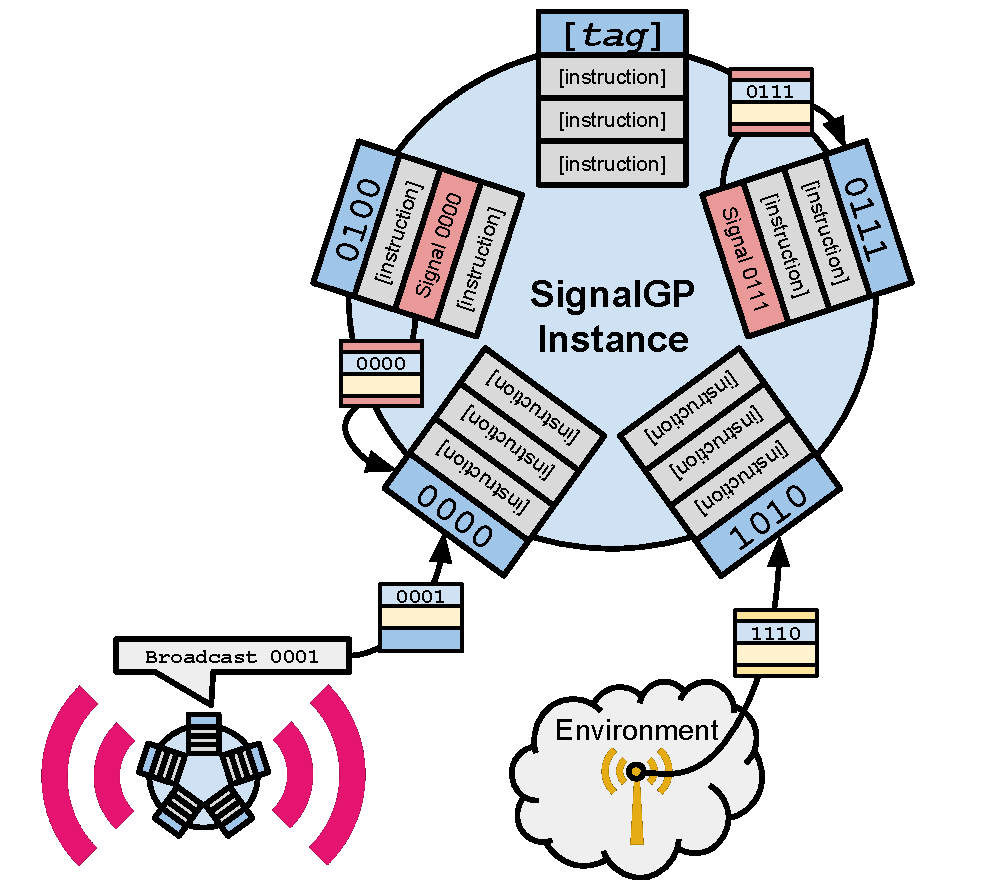
\includegraphics[width=\linewidth]{img/signalgp-cartoon}
{\textbf{(A)}
A cartoon overview of a single SignalGP instance.
SignalGP program modules execute pseudo-concurrently in response to tagged signals, which can originate internally, from the environment, or from other agents.
}
% \label{fig:signalgp-cartoon}
\end{minipage}
\end{minipage}%
% \hspace*{\fill}

% \hspace*{\fill}%
% \begin{minipage}[t]{\linewidth}
% \centering
% \vspace{0pt} % for alignment
% \begin{minipage}{\textwidth}
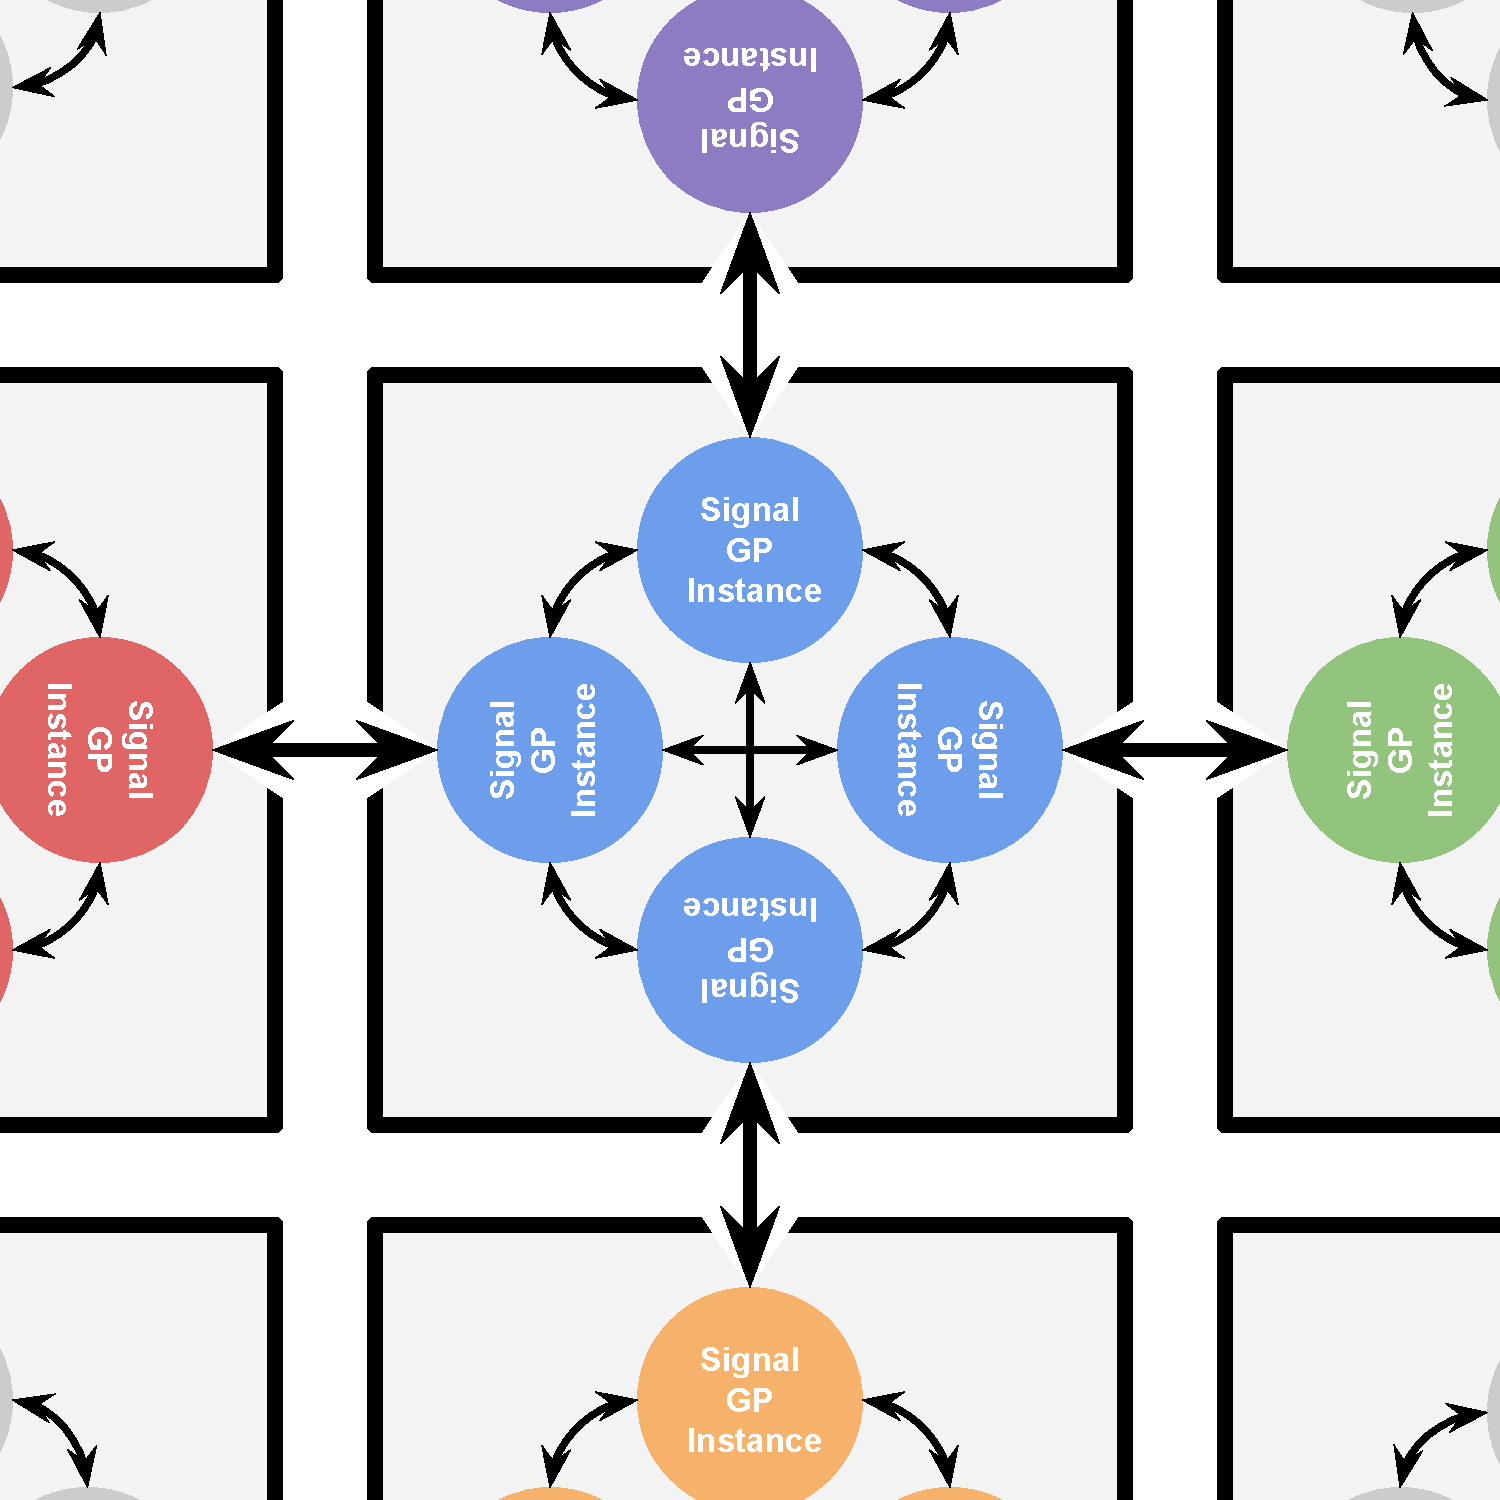
\includegraphics[width=0.8\linewidth]{img/dishtinygp-cartoon}\\
{\textbf{(B)}
A cartoon overview of how individual SignalGP instances are organized into DISHTINY cells.
% Each cell contains four independent SignalGP instances.
% The same genetic program is mirrored across all four SignalGP instances, but each instance executes independently.
Within each DISHTINY cell, each of four independent instances senses environmental state, receives intercellular messages, and determines cell behavior with respect to a single cardinal direction.
All four instances sense non-directional environmental cues and non-directional actions may be taken by any instance.
Instances within a cell communicate via intracellular messaging.
}
% \label{fig:dishtinygp-cartoon}
% \end{minipage}
% \end{minipage}%
% \hspace*{\fill}
\end{minipage}

\caption{
Schematic illustrations of how individual SignalGP instances function and how individual SignalGP instances are organized into DISHTINY cells.
Subfigure \textbf{(A)} provided courtesy Alexander Lalejini.
}
\label{fig:signalgp-dishtinygp}
\end{center}
\end{figure}


We performed simulations in which cells evolved open-ended behaviors to make decisions about resource sharing, reproductive timing, and apoptosis.
We will first describe the environment and hereditary grouping system cells evolved under and then describe the behavior-control system cells used.

\subsection{Cells and Hereditary Groups}

Cells occupy individual tiles on a 60-by-60 toroidal grid.
Over discrete time steps (``updates''), cells can collect a resource.
Collected resource decays at a rate of 0.1\% per update, incentivizing its quick use.
Once sufficient resource accrues, cells may pay one unit of resource to place a daughter cell on an adjoining tile of the toroidal grid (i.e., reproduce), replacing any existing cell already there.
Daughter cells inherit their parent's genetic program, except any novel mutations that may arise.
We used standard SignalGP mutation parameters from \citep{lalejini2018evolving}, but only applied mutations 1\% of daughter cells at birth.
Daughter cells may also inherit hereditary group ID, introduced and discussed below.

Cells accrue resource via a cooperative resource-collection process.
The simulation distributes large amounts of resource within certain spatial bounds in discrete, intermittent events.
Working in a group allows cells to more fully collect available resource during these events.
Cooperating in medium-sized groups (on the order of 100 cells) accelerates per-cell resource collection rate.
Unicellular, too-small, or too-large groups collect resource at a lesser per-cell rate.
As an arbitrary side effect of the simulation algorithm employed to instantiate the cooperative resource distribution process, groups with a roughly circular layout collect resource faster than irregularly-shaped groups.
Cooperative resource collection unfolds as an entirely passive process on the part of the cells, influenced only by a group's spatial layout.
Full details on the simulation algorithm that determines cooperative resource collection rates appear in in Supplementary Section \ref{sup:resource_collection_process}.

Cells may grow a cooperative resource-collecting group through cell proliferation.
We refer to these cooperative, resource-collecting groups as ``hereditary groups.''
As cells reproduce, they can choose to adsorb daughter cells onto the parent's hereditary group or expel those offspring to found a new hereditary group.
These decisions affect the spatial layout of these hereditary groups and, in turn, affect individual cells' resource-collection rate.

To promote group turnover, we counteract the advantage of established hereditary groups with a simple aging scheme.
As hereditary groups age over elapsed updates and somatic generations, their constituent cells lose the ability to regenerate somatic tissue and then, soon after, to collect resource.
A complete description of group aging mechanisms used appears in Supplementary Section \ref{sup:hereditary_group_life_cycle}.

Because new hereditary group IDs arise first in a single cell and grow disseminate exclusively among direct descendants of that progenitor cell, hereditary groups are reproductively bottlenecked.
This clonal (or ``staying together'') multicellular life history stands in contrast with an aggregative (or ``coming together'') life cycle where chimeric groups arise via fusion of potentially loosely-related lineages \citep{staps2019emergence}.
Such clonal development is known to strengthen between-organism selection effects \citep{grosberg2007evolution}.

In this work, we screen for fraternal transitions in individuality with respect to these hereditary groups by evaluating three characteristic traits of higher-level organisms: resource sharing, reproductive division of labor, and apoptosis.
We can further screen for the evolution of complex multicellularity by assessing cell-cell messaging, regulatory patterning, and functional differentiation between cells within hereditary groups \cite{knoll2011multiple}.

\subsection{Hierarchical Nesting of Hereditary Groups} \label{sec:hierarchical_nesting}

Successive fraternal transitions in natural history --- for example, to multicellularity and then to eusociality \citep{smith1997major} --- underscores the constructive power of evolution to harness emergent structures as building blocks for further novelty.
To explore these dynamics, in some experimental conditions we incorporated a hierarchical extension to the hereditary grouping scheme described above.

Hierarchical levels are introduced into the system by providing a mechanism to groups of hereditary groups to form.
We accomplish this through two separate, but overlaid, instantiations of the hereditary grouping scheme.
We refer to each independent hereditary grouping system as a ``level.''
The hierarchical extension allows two levels of hereditary grouping, identified here as L0 and L1.
Without the hierarchical extension, only L0 is present.
\footnote{
We chose to number these levels using the computer science convention of zero-based indexing (as opposed to everyday practice of counting up from one) to maintain consistency with source code and data sets associated with this work.
}
We refer to the highest hereditary grouping level present in a simulation as the ``apex'' level.

Under the hierarchical extension, each cell contained a pair of separate hereditary group IDs --- the first for L0 and the second for L1.
During reproduction, daughter cells could either
\begin{enumerate}
\item inherit both L0 and L1 hereditary group ID,
\item inherit L0 hereditary group ID but not L1 hereditary group ID, or
\item inherit neither hereditary group ID.
\end{enumerate}
In order to enforce hierarchical nesting of hereditary group IDs, daughter cells could not inherit just the L1 hereditary group ID.

Hierarchically hereditary group IDs are strictly nested: all cells are members of one L0 hereditary group and L1 hereditary group.
No cell can be a member of two L0 hereditary groups or two L1 hereditary groups.
Likewise, no L0 hereditary groups can appear within two different L1 hereditary groups.
Useful as a concrete illustration of this scheme, Figure \ref{fig:ko-morphology}\textbf{(A)} depicts hierarchically-nested hereditary groupings assumed by an evolved strain.

\subsection{Cell-Level Organisms}

Our experiments use cell-level digital organisms controlled by genetic programs subject to mutations and selective pressures that stem from local competition for limited space.

We employ the SignalGP event-driven genetic programming representation.
As sketched in Figure \ref{fig:signalgp-dishtinygp}\textbf{(A)}, this representation is specially designed to express function-like modules of code in response to internal signals or external stimuli.
This process can be considered somewhat akin to gene expression.
In our experiments, virtual CPUs can execute responses to up to 24 signals at once, with any further signals usurping the longest-running signal handlers.
The event-driven framework facilitates the evolution of dynamic interactions between digital organisms and their environment (including other organisms) \citep{lalejini2018evolving}.

Special module components allow evolving programs to sense and interact with their environment, through mechanisms including resource sharing, hereditary group sensing, apoptosis, cell reproduction, and arbitrary cell-cell messaging.
Modules can also include general purpose computational elements like conditionals and loops, which allows cells to evolve sophisticated behaviors conditioned on current (and even previous) local conditions.
A simple ``regulatory'' system provides special CPU instructions that dynamically adjust which modules are activated by particular signals.

Previous work evolving digital organisms in grid-based problem domains has relied on a single computational agent that designates a direction to act in via an explicit cardinal ``facing'' \citep{goldsby2014evolutionary, goldsby2018serendipitous, grabowski2010early, biswas2014causes, lalejini2018evolving}.
Here, we introduce novel methodology to facilitate the evolution of directionally-symmetric phenotypes.
In this work, each cell instantiates four copies of the SignalGP hardware: one facing each cardinal direction.
These hardware instances all execute the same SignalGP program and may coordinate via internal signals, but are otherwise decoupled.
Figure \ref{fig:signalgp-dishtinygp}\textbf{(B)} overviews the configuration of the four SignalGP instances that constitute a single cell.

Supplementary Sections \ref{sup:cell_level_organisms}, \ref{sup:standard_instruction_library}, \ref{sup:custom_instruction_library}, and \ref{sup:environmental_cue_library} provide full details of the digital evolution substrate underpinning this work.

\subsection{Surveyed Evolutionary Conditions}

To broaden our exploration of possible evolved multicellular behaviors in this system, we surveyed several evolutionary conditions.

In one manipulation, we explored the effect of structuring hereditary groups, such that parent cells can choose to keep offspring in their same sub-group, in just the same full group, or expel them entirely to start a new group.
Cells can independently mediate their behavior based on the level of the group with which they are interacting.

In a second manipulation, we explored the importance of explicitly selecting for medium-sized groups (as had been needed to maximize resource collection) by removing this incentive.
Instead, the system distributed resource at a uniform per-cell rate.

We combined these two manipulations to yield four surveyed conditions:
\begin{enumerate}
\item ``Flat-Even'': One hereditary group level (flat) with uniform resource inflow (even). In-browser simulation: \url{https://hopth.ru/i},
\item ``Flat-Wave'': One  hereditary group level (flat) with group-mediated resource collection (wave); In-browser simulation: \url{https://hopth.ru/j}),
\item ``Nested-Even'': Two hierarchically-nested hereditary group levels (nested) with uniform resource inflow (even). In-browser simulation: \url{https://hopth.ru/k},
\item ``Nested-Wave'': Two hierarchically-nested hereditary group levels (nested) with group-mediated resource collection (wave). In-browser simulation: \url{https://hopth.ru/l}.
\end{enumerate}

Supplementary Section \ref{sup:treatments} provides full details for each of the four surveyed evolutionary conditions.

For each condition, we simulated 40 replicate populations for up to
1,048,576 ($2^{20}$) updates.
During this time, on the order of 4,000 cellular generations and 500 apex-level group generations elapsed in runs.
(Full details appear in Supplementary Table \ref{sup:systematics}.)
Due to variability in simulation speed, four replicates only completed 262,144 updates.
All analyses involving inter-replicate comparisons were therefore performed at this earlier time point.


\section{Results}

To characterize the general selective pressures induced by surveyed environmental conditions, we assessed the prevalence of characteristic multicellular traits among evolved genotypes across replicates.
In the case of an evolutionary transition of individuality, we would expect cells to modulate their own reproductive behavior to prioritize group interests above individual cell interests.
In DISHTINY, cell reproduction inherently destroys an immediate neighbor cell.
As such, we would expect somatic growth to occur primarily at group peripheries in a higher-level individual.
Supplementary Figure \ref{fig:reproduction_surrounded} compares cellular reproduction rates between the interior and exterior of apex-level hereditary groups.
For all treatments, phenotypes with depressed interior cellular reproduction rates dominated across replicates (non-overlapping 95\% CI).
By update 262,144 (about 1,000 cellular generations; see Supplementary Table \ref{tab:systematics}), all four treatment conditions appear to select for some level of reproductive cooperation among cells.

Across replicate evolutionary runs in all four treatments, we also found that resource was transferred among registered kin at a significantly higher mean rate than to unrelated neighbors (non-overlapping 95\% CI).
Genetic programs controlling cells can sense whether any particular neighbor shares a common hereditary group ID.
Thus, selective activation of resource sharing behavior to hereditary group members might have evolved, which would provide one possible explanation for this observation.%
\footnote{%
Alternately to the same end, resource sharing behavior could be instead suppressed in the opposite case, when a neighbor holds a different hereditary group ID.
}
However, cells are also capable of conditioning behavior on whether a particular neighbor is direct kin (i.e., a parent or child).
To test whether this resource-sharing was solely an artifact of sharing between direct cellular kin, we also assessed mean sharing to registered kin that were not immediate cellular relatives.
Mean sharing between such cells also exceeded sharing among unrelated neighbors (non-overlapping 95\% CI).
Thus, all four treatments appear to select for functional cooperation among wider kin groups.
Supplementary section \ref{sec:resource-sharing} presents these results in detail.

\subsection{Qualitative Life Histories} \label{sec:life-histories}

\begin{figure*}[!htbp]
\begin{center}

\begin{minipage}[b]{\textwidth}
\centering
\begin{minipage}[t]{0.18\textwidth}
\centering
\adjincludegraphics[width=\textwidth, trim={{.5\width} {.33\width} {.17\width} {.38\width}}, clip]{img/lifecycle/naive-paint/seed=1026+title=directional_channel_grayscale_viz+treat=resource-wave__channelsense-yes__nlev-two+update=1048576+_data_hathash_hash=fdd6f7a5210124bd+_script_fullcat_hash=602c0d0c070e9202+_source_hash=53a2252-clean+ext=}
{\footnotesize Update 0}
\end{minipage}
\begin{minipage}[t]{0.18\textwidth}
\centering
\adjincludegraphics[width=\textwidth, trim={{.5\width} {.33\width} {.17\width} {.38\width}}, clip]{img/lifecycle/naive-paint/seed=1026+title=directional_channel_grayscale_viz+treat=resource-wave__channelsense-yes__nlev-two+update=1048704+_data_hathash_hash=fdd6f7a5210124bd+_script_fullcat_hash=602c0d0c070e9202+_source_hash=53a2252-clean+ext=}
{\footnotesize Update 128}
\end{minipage}
\begin{minipage}[t]{0.18\textwidth}
\centering
\adjincludegraphics[width=\textwidth, trim={{.5\width} {.33\width} {.17\width} {.38\width}}, clip]{img/lifecycle/naive-paint/seed=1026+title=directional_channel_grayscale_viz+treat=resource-wave__channelsense-yes__nlev-two+update=1048832+_data_hathash_hash=fdd6f7a5210124bd+_script_fullcat_hash=602c0d0c070e9202+_source_hash=53a2252-clean+ext=}
{\footnotesize Update 256}
\end{minipage}
\begin{minipage}[t]{0.18\textwidth}
\centering
\adjincludegraphics[width=\textwidth, trim={{.5\width} {.33\width} {.17\width} {.38\width}}, clip]{img/lifecycle/naive-paint/seed=1026+title=directional_channel_grayscale_viz+treat=resource-wave__channelsense-yes__nlev-two+update=1048960+_data_hathash_hash=fdd6f7a5210124bd+_script_fullcat_hash=602c0d0c070e9202+_source_hash=53a2252-clean+ext=}
{\footnotesize Update 384}
\end{minipage}
\begin{minipage}[t]{0.18\textwidth}
\centering
\adjincludegraphics[width=\textwidth, trim={{.5\width} {.33\width} {.17\width} {.38\width}}, clip]{img/lifecycle/naive-paint/seed=1026+title=directional_channel_grayscale_viz+treat=resource-wave__channelsense-yes__nlev-two+update=1049088+_data_hathash_hash=fdd6f7a5210124bd+_script_fullcat_hash=602c0d0c070e9202+_source_hash=53a2252-clean+ext=}
{\footnotesize Update 512}
\end{minipage}\\
\begin{minipage}{\textwidth}
\dissertationonly{\footnotesize}
\textbf{(A)}
Naive
(%
animation: \url{https://hopth.ru/x},
in-browser simulation: \url{https://hopth.ru/1}%
).
The offspring group is birthed at the exterior of the parent group.
Parent and offspring groups then compete with each other for space just the same as they do with other groups.
\end{minipage}
% \label{fig:lifecycle-naive}
\end{minipage}

\vspace{3ex}

\begin{minipage}[b]{\textwidth}
\centering
\begin{minipage}[t]{0.18\textwidth}
\centering
\adjincludegraphics[width=\textwidth, trim={{.66\width} {.71\width} {.0\width} {.0\width}}, clip]{img/lifecycle/adjoin-paint/seed=1004+title=directional_channel_grayscale_viz+treat=resource-wave__channelsense-yes__nlev-two+update=1048896+_data_hathash_hash=51fd4923ae7e3bde+_script_fullcat_hash=602c0d0c070e9202+_source_hash=53a2252-clean+ext=}
{\footnotesize Update 0}
\end{minipage}
\begin{minipage}[t]{0.18\textwidth}
\centering
\adjincludegraphics[width=\textwidth, trim={{.66\width} {.71\width} {.0\width} {.0\width}}, clip]{img/lifecycle/adjoin-paint/seed=1004+title=directional_channel_grayscale_viz+treat=resource-wave__channelsense-yes__nlev-two+update=1048928+_data_hathash_hash=51fd4923ae7e3bde+_script_fullcat_hash=602c0d0c070e9202+_source_hash=53a2252-clean+ext=}
{\footnotesize Update 32}
\end{minipage}
\begin{minipage}[t]{0.18\textwidth}
\centering
\adjincludegraphics[width=\textwidth, trim={{.66\width} {.71\width} {.0\width} {.0\width}}, clip]{img/lifecycle/adjoin-paint/seed=1004+title=directional_channel_grayscale_viz+treat=resource-wave__channelsense-yes__nlev-two+update=1048960+_data_hathash_hash=51fd4923ae7e3bde+_script_fullcat_hash=602c0d0c070e9202+_source_hash=53a2252-clean+ext=}
{\footnotesize Update 64}
\end{minipage}
\begin{minipage}[t]{0.18\textwidth}
\centering
\adjincludegraphics[width=\textwidth, trim={{.66\width} {.71\width} {.0\width} {.0\width}}, clip]{img/lifecycle/adjoin-paint/seed=1004+title=directional_channel_grayscale_viz+treat=resource-wave__channelsense-yes__nlev-two+update=1049024+_data_hathash_hash=51fd4923ae7e3bde+_script_fullcat_hash=602c0d0c070e9202+_source_hash=53a2252-clean+ext=}
{\footnotesize Update 128}
\end{minipage}
\begin{minipage}[t]{0.18\textwidth}
\centering
\adjincludegraphics[width=\textwidth, trim={{.66\width} {.71\width} {.0\width} {.0\width}}, clip]{img/lifecycle/adjoin-paint/seed=1004+title=directional_channel_grayscale_viz+treat=resource-wave__channelsense-yes__nlev-two+update=1049408+_data_hathash_hash=51fd4923ae7e3bde+_script_fullcat_hash=602c0d0c070e9202+_source_hash=53a2252-clean+ext=}
{\footnotesize Update 512}
\end{minipage}\\
\begin{minipage}{\textwidth}
\dissertationonly{\footnotesize}
\textbf{(B)} Adjoin
(%
animation: \url{https://hopth.ru/y},
in-browser simulation: \url{https://hopth.ru/2}%
).
The offspring group begins as a single cell at the exterior of the parent group.
Parent and offspring groups then exclusively expend reproductive effort to compete with other groups.
This results in a stable interface between the parent and offspring groups as the offspring group grows over time.
\end{minipage}
% \label{fig:lifecycle-adjoin}
\end{minipage}

\vspace{3ex}

\begin{minipage}[b]{\textwidth}
\centering
\begin{minipage}[t]{0.18\textwidth}
\centering
\adjincludegraphics[width=\textwidth, trim={{.0\width} {.05\width} {.66\width} {.66\width}}, clip]{img/lifecycle/sweep-paint/seed=1023+title=directional_channel_grayscale_viz+treat=resource-wave__channelsense-yes__nlev-two+update=1048648+_data_hathash_hash=519a2d5a19f16020+_script_fullcat_hash=602c0d0c070e9202+_source_hash=53a2252-clean+ext=}
{\footnotesize Update 0}
\end{minipage}
\begin{minipage}[t]{0.18\textwidth}
\centering
\adjincludegraphics[width=\textwidth, trim={{.0\width} {.05\width} {.66\width} {.66\width}}, clip]{img/lifecycle/sweep-paint/seed=1023+title=directional_channel_grayscale_viz+treat=resource-wave__channelsense-yes__nlev-two+update=1048720+_data_hathash_hash=519a2d5a19f16020+_script_fullcat_hash=602c0d0c070e9202+_source_hash=53a2252-clean+ext=}
{\footnotesize Update 72}
\end{minipage}
\begin{minipage}[t]{0.18\textwidth}
\centering
\adjincludegraphics[width=\textwidth, trim={{.0\width} {.05\width} {.66\width} {.66\width}}, clip]{img/lifecycle/sweep-paint/seed=1023+title=directional_channel_grayscale_viz+treat=resource-wave__channelsense-yes__nlev-two+update=1048792+_data_hathash_hash=519a2d5a19f16020+_script_fullcat_hash=602c0d0c070e9202+_source_hash=53a2252-clean+ext=}
{\footnotesize Update 144}
\end{minipage}
\begin{minipage}[t]{0.18\textwidth}
\centering
\adjincludegraphics[width=\textwidth, trim={{.0\width} {.05\width} {.66\width} {.66\width}}, clip]{img/lifecycle/sweep-paint/seed=1023+title=directional_channel_grayscale_viz+treat=resource-wave__channelsense-yes__nlev-two+update=1048864+_data_hathash_hash=519a2d5a19f16020+_script_fullcat_hash=602c0d0c070e9202+_source_hash=53a2252-clean+ext=}
{\footnotesize Update 216}
\end{minipage}
\begin{minipage}[t]{0.18\textwidth}
\centering
\adjincludegraphics[width=\textwidth, trim={{.0\width} {.05\width} {.66\width} {.66\width}}, clip]{img/lifecycle/sweep-paint/seed=1023+title=directional_channel_grayscale_viz+treat=resource-wave__channelsense-yes__nlev-two+update=1048936+_data_hathash_hash=519a2d5a19f16020+_script_fullcat_hash=602c0d0c070e9202+_source_hash=53a2252-clean+ext=}
{\footnotesize Update 288}
\end{minipage}\\
\begin{minipage}{\textwidth}
\dissertationonly{\footnotesize}
\textbf{(C)} Sweep
(%
animation: \url{https://hopth.ru/z},
in-browser simulation: \url{https://hopth.ru/3}%
).
The offspring group begins as a single cell at the exterior of the parent group.
The offspring group then grows rapidly into the parent group, resulting in a near-complete transfer of simulation space into the offspring group.
Multiple offspring groups may simultaneously grow over the parent, as is the case here.
\end{minipage}
% \label{fig:lifecycle-sweep}
\end{minipage}

\vspace{3ex}

\begin{minipage}[b]{\textwidth}
\centering
\begin{minipage}[t]{0.18\textwidth}
\centering
\adjincludegraphics[width=\textwidth, trim={{.0\width} {.71\width} {.66\width} {.0\width}}, clip]{img/lifecycle/burst-paint/seed=1034+title=directional_channel_grayscale_viz+treat=resource-wave__channelsense-yes__nlev-two+update=1048648+_data_hathash_hash=ca8ad21d3b30b939+_script_fullcat_hash=602c0d0c070e9202+_source_hash=53a2252-clean+ext=}
{\footnotesize Update 0}
\end{minipage}
\begin{minipage}[t]{0.18\textwidth}
\centering
\adjincludegraphics[width=\textwidth, trim={{.0\width} {.71\width} {.66\width} {.0\width}}, clip]{img/lifecycle/burst-paint/seed=1034+title=directional_channel_grayscale_viz+treat=resource-wave__channelsense-yes__nlev-two+update=1048744+_data_hathash_hash=ca8ad21d3b30b939+_script_fullcat_hash=602c0d0c070e9202+_source_hash=53a2252-clean+ext=}
{\footnotesize Update 96}
\end{minipage}
\begin{minipage}[t]{0.18\textwidth}
\centering
\adjincludegraphics[width=\textwidth, trim={{.0\width} {.71\width} {.66\width} {.0\width}}, clip]{img/lifecycle/burst-paint/seed=1034+title=directional_channel_grayscale_viz+treat=resource-wave__channelsense-yes__nlev-two+update=1048840+_data_hathash_hash=ca8ad21d3b30b939+_script_fullcat_hash=602c0d0c070e9202+_source_hash=53a2252-clean+ext=}
{\footnotesize Update 192}
\end{minipage}
\begin{minipage}[t]{0.18\textwidth}
\centering
\adjincludegraphics[width=\textwidth, trim={{.0\width} {.71\width} {.66\width} {.0\width}}, clip]{img/lifecycle/burst-paint/seed=1034+title=directional_channel_grayscale_viz+treat=resource-wave__channelsense-yes__nlev-two+update=1048936+_data_hathash_hash=ca8ad21d3b30b939+_script_fullcat_hash=602c0d0c070e9202+_source_hash=53a2252-clean+ext=}
{\footnotesize Update 288}
\end{minipage}
\begin{minipage}[t]{0.18\textwidth}
\centering
\adjincludegraphics[width=\textwidth, trim={{.0\width} {.71\width} {.66\width} {.0\width}}, clip]{img/lifecycle/burst-paint/seed=1034+title=directional_channel_grayscale_viz+treat=resource-wave__channelsense-yes__nlev-two+update=1049032+_data_hathash_hash=ca8ad21d3b30b939+_script_fullcat_hash=602c0d0c070e9202+_source_hash=53a2252-clean+ext=}
{\footnotesize Update 384}
\end{minipage}\\
\begin{minipage}{\textwidth}
\dissertationonly{\footnotesize}
\textbf{(D)} Burst
(%
animation: \url{https://hopth.ru/0},
in-browser simulation: \url{https://hopth.ru/4}%
).
The offspring group begins as a single cell at the interior of the parent group.
Over time, the offspring group grows over the parent group from the inside out.
Multiple offspring groups may develop simultaneously, as is the case here.
\end{minipage}
% \label{fig:lifecycle-burst}
\end{minipage}

\caption{
Time lapse examples of qualitative life histories evolved under the Nested-Wave treatment.
From left to right within each row, frames depict the progression of simulation state within a subset of the simulation grid.
L1 hereditary groups are by differentiated by grayscale tone and separated by solid black borders.
L0 hereditary groups are by separated by dashed gray borders.
In each example, the focal parent L1 group is colored purple and the focal offspring group orange.
}
\label{fig:lifecycle}
\end{center}
\end{figure*}


Although cooperative cell-level phenotypes were common among evolved hereditary groups, across replicates functional and reproductive cooperation arose via diverse qualitative life histories.
To provide a general sense for the types of life histories we observed in this system, Figure \ref{fig:lifecycle} shows time lapses of representative multicellular groups evolved in different replicates.
Figure \ref{fig:lifecycle}\textbf{(A)} depicts an example of a naive life history in which --- beyond the cellular progenitor of a propagule group --- the parent and propagule groups exhibit no special cooperative relationship.
In Figure \ref{fig:lifecycle}\textbf{(B)}, propagules repeatedly bud off of parent groups to yield a larger network of persistent parent-child cooperators.
In Figure \ref{fig:lifecycle}\textbf{(C)}, propagules are generated at the extremities of parent groups and then rapidly replace most or all of the parent group.
Finally, in Figure \ref{fig:lifecycle}\textbf{(D)}, propagules are generated at the interior of a parent group and replace it from the inside out.

To better understand the multicellular strategies that evolved in this system, we investigated the mechanisms and adaptiveness of notable phenotypes that evolved in several individual evolutionary replicates.
In the following sections, we present these investigations as a series of case studies.

%Section \ref{sec:gene-regulation} reports a particular group-replication strategy in which propagule groups are seeded within the soma, destroying the parent as they mature.


\subsection{Case Study: Burst Lifecycle} \label{sec:gene-regulation}

\begin{figure}[!htbp]
\begin{center}

\begin{minipage}[t]{0.5\linewidth}

% \begin{minipage}[b]{\linewidth}
% \begin{center}

% \begin{minipage}[t]{0.18\linewidth}
% \centering
% \vspace{0pt} % for alignment
% \adjincludegraphics[width=\textwidth, trim={{.0\width} {.77\width} {.79\width} {.02\width}}, clip]{img/lifecycle/burst-paint/seed=1034+title=directional_channel_grayscale_viz+treat=resource-wave__channelsense-yes__nlev-two+update=1048648+_data_hathash_hash=ca8ad21d3b30b939+_script_fullcat_hash=602c0d0c070e9202+_source_hash=53a2252-clean+ext=}
% \footnotesize Update 0
% \end{minipage}
% \begin{minipage}[t]{0.18\linewidth}
% \centering
% \vspace{0pt} % for alignment
% \adjincludegraphics[width=\textwidth, trim={{.0\width} {.77\width} {.79\width} {.02\width}}, clip]{img/lifecycle/burst-paint/seed=1034+title=directional_channel_grayscale_viz+treat=resource-wave__channelsense-yes__nlev-two+update=1048744+_data_hathash_hash=ca8ad21d3b30b939+_script_fullcat_hash=602c0d0c070e9202+_source_hash=53a2252-clean+ext=}
% \footnotesize 96
% \end{minipage}
% \begin{minipage}[t]{0.18\linewidth}
% \centering
% \vspace{0pt} % for alignment
% \adjincludegraphics[width=\textwidth, trim={{.0\width} {.77\width} {.79\width} {.02\width}}, clip]{img/lifecycle/burst-paint/seed=1034+title=directional_channel_grayscale_viz+treat=resource-wave__channelsense-yes__nlev-two+update=1048840+_data_hathash_hash=ca8ad21d3b30b939+_script_fullcat_hash=602c0d0c070e9202+_source_hash=53a2252-clean+ext=}
% \footnotesize 192
% \end{minipage}
% \begin{minipage}[t]{0.18\linewidth}
% \centering
% \vspace{0pt} % for alignment
% \adjincludegraphics[width=\textwidth, trim={{.0\width} {.77\width} {.79\width} {.02\width}}, clip]{img/lifecycle/burst-paint/seed=1034+title=directional_channel_grayscale_viz+treat=resource-wave__channelsense-yes__nlev-two+update=1048936+_data_hathash_hash=ca8ad21d3b30b939+_script_fullcat_hash=602c0d0c070e9202+_source_hash=53a2252-clean+ext=}
% \footnotesize 288
% \end{minipage}
% \begin{minipage}[t]{0.18\linewidth}
% \centering
% \vspace{0pt} % for alignment
% \adjincludegraphics[width=\textwidth, trim={{.0\width} {.77\width} {.79\width} {.02\width}}, clip]{img/lifecycle/burst-paint/seed=1034+title=directional_channel_grayscale_viz+treat=resource-wave__channelsense-yes__nlev-two+update=1049032+_data_hathash_hash=ca8ad21d3b30b939+_script_fullcat_hash=602c0d0c070e9202+_source_hash=53a2252-clean+ext=}
% \footnotesize 384
% \end{minipage}
% \caption{Wild type timelapse}
% \label{fig:wt_timelapse}
% \end{center}
% \end{minipage}

% \vspace{2ex}

\begin{minipage}[b]{\linewidth}
\begin{center}

\begin{minipage}[t]{0.30\linewidth}
\centering
\vspace{0pt} % for alignment
% adapted from https://tex.stackexchange.com/a/186476
\begin{tikzpicture}
\node[anchor=south west,inner sep=0] (image) at (0,0) { \adjincludegraphics[width=\linewidth, trim={{.25\width} {.20\width} {.5\width} {.55\width}}, clip]{img/knockout/interior_propagule/wildtype/retouched3_seed=1+title=directional_regulator_viz+treat=resource-wave__channelsense-yes__nlev-two+update=8188+_data_hathash_hash=8b493febd79aad1f+_script_fullcat_hash=90718bb0c6ec4dbd+_source_hash=53a2252-clean+ext=}
};
\begin{scope}[x={(image.south east)},y={(image.north west)}]
  \draw [ultra thick,-{stealth[scale=1.25]}, white] (0.35,0.59) -- ++(0.06,-0.06);
  \draw [ultra thick, -{stealth[scale=1.25]}, white] (0.01,0.39) -- ++(0.06,-0.06);
  \draw [ultra thick, -{stealth[scale=1.25]}, white] (0.68,0.39) -- ++(0.06,-0.06);
  \draw [ultra thick, -{stealth[scale=1.25]}, white] (0.62,0.32) -- ++(0.06,-0.06);
  \draw [-stealth, red] (0.35,0.59) -- ++(0.05,-0.05);
  \draw [-stealth, red] (0.01,0.39) -- ++(0.05,-0.05);
  \draw [-stealth, red] (0.68,0.39) -- ++(0.05,-0.05);
  \draw [-stealth, red] (0.62,0.32) -- ++(0.05,-0.05);
\end{scope}
\end{tikzpicture}
\footnotesize Wild type
\end{minipage}
\begin{minipage}[t]{0.30\linewidth}
\centering
\vspace{0pt} % for alignment
\adjincludegraphics[width=\linewidth, trim={{.5\width} {.5\width} {.25\width} {.25\width}}, clip]{img/knockout/interior_propagule/propaguleknockout/retouched2_seed=1+title=directional_regulator_viz+treat=resource-wave__channelsense-yes__nlev-two+update=8188+_data_hathash_hash=2b6711db47fb5887+_script_fullcat_hash=90718bb0c6ec4dbd+_source_hash=53a2252-clean+ext=}
\footnotesize Propagule knockout
\end{minipage}
\begin{minipage}[t]{0.30\linewidth}
\centering
\vspace{0pt} % for alignment
\adjincludegraphics[width=\linewidth, trim={{.5\width} {.5\width} {.25\width} {.25\width}}, clip]{img/knockout/interior_propagule/regulationknockout/retouched_seed=1+title=directional_regulator_viz+treat=resource-wave__channelsense-yes__nlev-two+update=8188+_data_hathash_hash=11ab5cdd47ed18c7+_script_fullcat_hash=90718bb0c6ec4dbd+_source_hash=53a2252-clean+ext=}
\footnotesize Regulation knockout
\end{minipage}

{\textbf{(A)} Regulation visualizations}
% \label{fig:regulation_visualizations}

\end{center}
\end{minipage}

\begin{minipage}[t]{\linewidth}
\centering
\vspace{0pt} % for alignment
\begin{minipage}[b]{\linewidth}
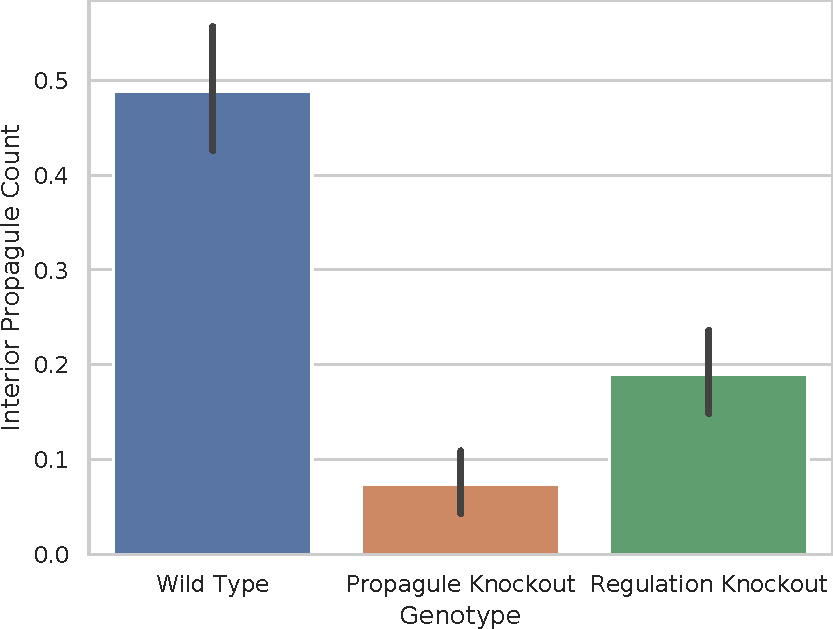
\includegraphics[width=\linewidth]{img/knockout/interior_propagule/title=interior_propagules+_data_hathash_hash=bb0fa6254f1b7398+_script_fullcat_hash=f738b363bea8c98a+_source_hash=53a2252-clean+ext=}
{\textbf{(B)} Interior propagule rate by genotype}
% \label{fig:interior_propagule_rate}
\end{minipage}
\end{minipage}%
\hspace*{\fill}

\end{minipage}

\caption{
Analysis of a wild type strain exhibiting a ``burst'' lifecycle evolved under the ``Nested-Wave'' treatment exhibiting interior propagule generation.
% Figure \ref{fig:wt_timelapse} traces the wild type life history.
% L1 hereditary groups are by differentiated by grayscale tone and separated by solid black borders.
% L0 hereditary groups are by separated by gray borders.
% In each example, the focal parent L1 hereditary group is colored purple and the focal offspring group orange.
Subfigure \textbf{(A)} compares gene regulation between analyzed strains.
Group layouts are overlaid via borders between cells.
Black borders divide L1 groups and white borders divide L0 groups.
Borders between L1 groups are underlined in red for greater visibility.
state for each cell's four directional SignalGP instances.
Within these group layouts, regulation state for each cell's four directional SignalGP instances is color coded using a PCA mapping from regulatory state to three-dimensional RGB coordinates.
(The PCA mapping is calculated uniquely for each L1 hereditary group.)
Within a L1 hereditary group, color similarity among tile quarters indicates that the corresponding SignalGP instances exhibit similar regulatory state.
In the case of identical regulatory state (here, due to the absence of genetic regulation in a knockout strain) this color coding appears gray.
Wild type interior propagules are annotated with red arrows.
Subfigure \textbf{(B)} compares the mean number of interior propagules observed per L1 hereditary group.
Error bars indicate 95\% confidence.
View an animation of wild type gene regulation at \url{https://hopth.ru/t}.
View the wild type strain in a live in-browser simulation at \url{https://hopth.ru/g}.
}
\label{fig:ko-interior_propagule}
\end{center}
\end{figure}


%This wild type strain exhibits an irregular, but somewhat concentric, spatial pattern of gene regulation illustrated in Figure \ref{fig:ko-interior_propagule}\textbf{(A)}.
%In time-series animation, linked in the figure caption, gene regulation appears to fluctuate dynamically.

We wondered how the strain exhibiting the ``burst'' lifecycle in Figure \ref{fig:lifecycle}\textbf{(D)} determined when and where to originate its propagules.
To assess whether gene regulation instructions played a role in this process, we prepared two knockout strains.
In the first, gene regulation instructions were replaced with no-operation (Nop) instructions (so that gene regulation state would remain baseline).
In the second, the reproduction instructions to spawn a propagule were replaced with Nop instructions.
Figure \ref{fig:ko-interior_propagule}\textbf{(A)} depicts the gene regulation phenotypes of these strains.

Figure \ref{fig:ko-interior_propagule}\textbf{(B)} compares interior propagule generation between the strains, confirming the direct mechanistic role of gene regulation in promoting interior propagule generation (non-overlapping 95\% CI).

In head-to-head match-ups, the wild type strain outcompetes both the regulation-knockout ($20/20$; $p < 0.001$; two-tailed Binomial test) and the propagule-knockout strains
($20/20$; $p < 0.001$; two-tailed Binomial test).
The deficiency of the propagule-knockout strain confirms the adaptive role of interior propagule generation.
Likewise, the deficiency of the regulation-knockout strain affirms the adaptive role of gene regulation in the focal wild type strain.

\subsection{Case Study: Cell-cell Messaging} \label{sec:cell-cell-messaging}

\begin{figure}[!htbp]
\begin{center}

\begin{minipage}[t]{0.5\linewidth}

\begin{minipage}[t]{\linewidth}
\hspace*{\fill}%
\begin{minipage}[t]{0.05\linewidth}
\vspace{0pt} % for alignment
\rotatebox{90}{Messaging}%
\end{minipage}%
\hfill
\begin{minipage}[t]{0.45\linewidth}
\centering
\vspace{0pt} % for alignment
\adjincludegraphics[width=\textwidth, trim={{.0\width} {.0\width} {.5\width} {.5\width}}, clip]{img/knockout/intermessaging-sharing/wildtype/seed=1+title=directional_messaging_viz+treat=resource-wave__channelsense-yes__nlev-onebig+update=7172+_data_hathash_hash=f9e2a8ff33bf7745+_script_fullcat_hash=6b7e0389992dd616+_source_hash=53a2252-clean+ext=}%
\end{minipage}%
\hfill
\begin{minipage}[t]{0.45\linewidth}
\centering
\vspace{0pt} % for alignment
\adjincludegraphics[width=\textwidth, trim={{.0\width} {.0\width} {.5\width} {.5\width}}, clip]{img/knockout/intermessaging-sharing/knockout/seed=1+title=directional_messaging_viz+treat=resource-wave__channelsense-yes__nlev-onebig+update=7172+_data_hathash_hash=ffdeb1c77dd012e1+_script_fullcat_hash=6b7e0389992dd616+_source_hash=53a2252-clean+ext=}%
\end{minipage}%
\hspace*{\fill}

\hspace*{\fill}%
\begin{minipage}[t]{0.05\linewidth}
\vspace{0pt} % for alignment
\rotatebox{90}{Resource Sharing}%
\end{minipage}%
\hfill
\begin{minipage}[t]{0.45\linewidth}
\centering
\vspace{0pt} % for alignment
\adjincludegraphics[width=\textwidth, trim={{.0\width} {.0\width} {.5\width} {.5\width}}, clip]{img/knockout/intermessaging-sharing/wildtype/seed=1+title=directional_sharing_viz+treat=resource-wave__channelsense-yes__nlev-onebig+update=7172+_data_hathash_hash=f9e2a8ff33bf7745+_script_fullcat_hash=3a1e851383e0ffd4+_source_hash=53a2252-clean+ext=}%
\end{minipage}%
\hfill
\begin{minipage}[t]{0.45\linewidth}
\centering
\vspace{0pt} % for alignment
\adjincludegraphics[width=\textwidth, trim={{.0\width} {.0\width} {.5\width} {.5\width}}, clip]{img/knockout/intermessaging-sharing/knockout/seed=1+title=directional_sharing_viz+treat=resource-wave__channelsense-yes__nlev-onebig+update=7172+_data_hathash_hash=ffdeb1c77dd012e1+_script_fullcat_hash=3a1e851383e0ffd4+_source_hash=53a2252-clean+ext=}%
\end{minipage}%
\hspace*{\fill}

\hspace*{\fill}%
\begin{minipage}[t]{0.05\linewidth}
\vspace{0pt} % for alignment
\rotatebox{90}{Resource Stockpile}%
\end{minipage}%
\hfill
\begin{minipage}[t]{0.45\linewidth}
\centering
\vspace{0pt} % for alignment
\adjincludegraphics[width=\textwidth, trim={{.0\width} {.0\width} {.5\width} {.5\width}}, clip]{img/knockout/intermessaging-sharing/wildtype/seed=1+title=stockpile_viz+treat=resource-wave__channelsense-yes__nlev-onebig+update=7172+_data_hathash_hash=f9e2a8ff33bf7745+_script_fullcat_hash=4c8152cbf92e0da6+_source_hash=53a2252-clean+ext=}%
\end{minipage}%
\hfill
\begin{minipage}[t]{0.45\linewidth}
\centering
\vspace{0pt} % for alignment
\adjincludegraphics[width=\textwidth, trim={{.0\width} {.0\width} {.5\width} {.5\width}}, clip]{img/knockout/intermessaging-sharing/knockout/seed=1+title=stockpile_viz+treat=resource-wave__channelsense-yes__nlev-onebig+update=7172+_data_hathash_hash=ffdeb1c77dd012e1+_script_fullcat_hash=4c8152cbf92e0da6+_source_hash=53a2252-clean+ext=}%
\end{minipage}%
\hspace*{\fill}

\vspace{1.0ex}

\hspace*{\fill}%
\begin{minipage}[t]{0.05\linewidth}
\vspace{0pt} % for alignment
\end{minipage}%
\hfill
\begin{minipage}[t]{0.45\linewidth}
\centering
\vspace{0pt} % for alignment
Wild Type
\end{minipage}%
\hfill
\begin{minipage}[t]{0.45\linewidth}
\centering
\vspace{0pt} % for alignment
Messaging Knockout
\end{minipage}%
\hspace*{\fill}

\vspace{1.0ex}

% \begin{minipage}{\linewidth}
%   \caption{Phenotype visualizations}
%   \label{fig:intermessaging-sharing-phen}
% \end{minipage}

\end{minipage}%
% \begin{minipage}[t]{\linewidth}
%
% \hspace*{\fill}%
% \begin{minipage}[t]{\textwidth}
% \centering
% \vspace{0pt} % for alignment
% \begin{minipage}[b]{\textwidth}
% \includegraphics[width=\textwidth]{img/knockout/intermessaging-sharing/title=sharingdirection+_data_hathash_hash=59f6520a17fb3ad8+_script_fullcat_hash=97aad8dce5e50084+_source_hash=53a2252-clean+ext=}%
% \caption{Net sharing direction variance}
% \label{fig:intermessaging-sharing-direction}
% \end{minipage}
% \end{minipage}%
% \hfill
% \begin{minipage}[t]{\textwidth}
% \centering
% \vspace{0pt} % for alignment
% \begin{minipage}[b]{\textwidth}
% 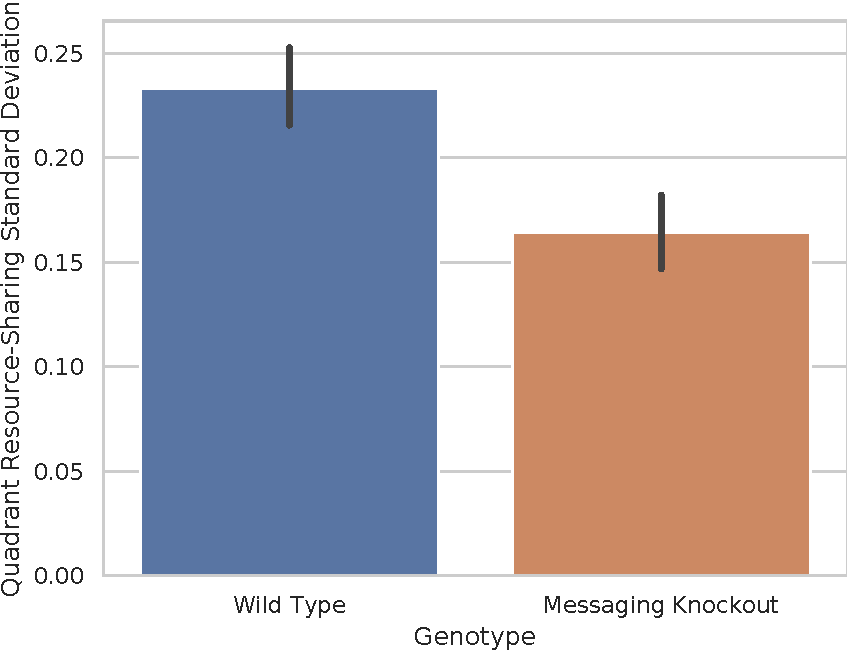
\includegraphics[width=\textwidth]{img/knockout/intermessaging-sharing/title=sharingquadrant+_data_hathash_hash=586f3c805332c323+_script_fullcat_hash=6e8aa37a96d9d7a9+_source_hash=53a2252-clean+ext=}%
% \caption{Net sharing localization variance}
% \label{fig:intermessaging-sharing-quadrant}
% \end{minipage}
% \end{minipage}%
% \hfill
% \begin{minipage}[t]{\textwidth}
% \centering
% \vspace{0pt} % for alignment
% \begin{minipage}[b]{\textwidth}
% \includegraphics[width=\textwidth]{img/knockout/intermessaging-sharing/title=fractionresevoir+_data_hathash_hash=7ce9af7e8fe0699b+_script_fullcat_hash=da31ee3af7ae0208+_source_hash=53a2252-clean+ext=}%
% \caption{Fraction of cells with enough resource to reproduce}
% \label{fig:intermessaging-sharing-resevoir}
% \end{minipage}
% \end{minipage}%
% \hspace*{\fill}
% \end{minipage}

\end{minipage}

\caption{
Visualization of phenotypic traits of a wild type strain evolved under the ``Flat-Wave'' treatment and corresponding intercell messaging knockout strain.
For these visualizations, group layouts are overlaid via borders between cells.
Black borders divide L0 hereditary groups.
In the messaging visualization, color coding represents the volume of incoming messages.
White represents no incoming messages and the magenta to blue gradient runs from one incoming message to the maximum observed incoming message traffic.
Unlike the wild type strain, as expected the messaging knockout strain exhibits no messaging activity.
In the resource sharing visualization, color coding represents the amount of incoming resource.
White represents no incoming resource and the magenta to blue gradient runs from the minimum to the maximum observed incoming incoming resource.
The wild type strain exhibits much more sparse resource sharing than the messaging knockout strain.
In the resource stockpile visualization, white represents zero-resource stockpiles, blue represents stockpiles with just under enough resource to reproduce, green represents stockpiles with enough resource to reproduce, and yellow represents more than enough resource to reproduce.
The wild type groups contain more cells with rich resource stockpiles (green and yellow) than the messaging knockout strain.
View an animation of the wild type strain at \url{https://hopth.ru/p}.
View the wild type strain in a live in-browser simulation at \url{https://hopth.ru/e}.
% minipages \ref{fig:intermessaging-sharing-direction}, \ref{fig:intermessaging-sharing-quadrant}, \ref{fig:intermessaging-sharing-resevoir} quantify knockout effects on various phenotypic traits.
% Error bars indicate 95\% confidence.
}
\label{fig:ko-intermessaging-sharing}
\end{center}
\end{figure}


We discovered adaptive cell-cell messaging in two evolved strains.
Here, we discuss a strain evolved under the Flat-Wave treatment where cell-cell messaging disrupts directional and spatial uniformity of resource sharing.
Supplementary Section \ref{sec:intergroup} overviews an evolved strain where cell-cell messaging appears to intensify expression of a contextual tit-for-tat policy between hereditary groups.

Figure \ref{fig:ko-intermessaging-sharing} depicts the cell-cell messaging, resource sharing, and resource stockpile phenotypes of the wild type strain side-by-side with corresponding phenotypes of a cell-cell messaging knockout strain.
In the wild type strain, cell-cell messaging emanates from irregular collection of cells --- in some regions, grid-like and in others more sparse --- broadcasting to all neighboring cells.
Resource sharing appears more widespread in the knockout strain than in the wild type.
However, messaging's effects suppressing resource sharing is neither spatially nor directionally homogeneous.
Relative to the knockout strain, cell-cell messaging increases variance in cardinal directionality of net resource sharing
(%
WT: mean 0.28, S.D. 0.07, $n=54$; % 2020/01-06-ll.md
KO: mean 0.17, S.D. 0.07, $n=69$; % 2020/01-06-ll.md
%Figure \ref{fig:intermessaging-sharing-direction};
$p < 0.001$, bootstrap test%
).
Cell-cell messaging also increases variance of resource sharing density with respect to spatial quadrants demarcated by the hereditary group's spatial centroid
(%
WT: mean 0.23, S.D. 0.07, $n=52$; % 2020/01-06-ll.md
KO: mean 0.16, S.D. 0.08, $n=68$; % 2020/01-06-ll.md
%Figure \ref{fig:intermessaging-sharing-quadrant};
$p < 0.001$, bootstrap test% 2020/01-06-ll.md
).
We used competition experiments to confirm the fitness advantage both of cell-cell messaging ($20/20$; $p < 0.001$; two-tailed Binomial test) and (using a separate knockout strain) resource sharing ($20/20$; $p < 0.001$; two-tailed Binomial test).
The fitness advantage of irregularized sharing might stem from a corresponding increase in the fraction of cells with enough resource to reproduce stockpiled
(%
WT: mean 0.18, S.D. 0.11, $n=54$; % 2020/01-06-ll.md
KO: mean 0.06, S.D. 0.08, $n=69$; % 2020/01-06-ll.md
$p < 0.001$, bootstrap test% 2020/01-06-ll.md
).

\subsection{Case Study: Gradient-conditioned Cell Behavior} \label{sec:gradient-conditioned-behavior}

\begin{figure}[!htbp]
\begin{center}

\centering

\hspace*{\fill}%
\begin{minipage}[t]{0.05\columnwidth}
\vspace{0pt} % for alignment
\rotatebox{90}{Resource Stockpile}%
\end{minipage}%
\hfill
\begin{minipage}[t]{0.45\columnwidth}
\centering
\vspace{0pt} % for alignment
\adjincludegraphics[width=\textwidth, trim={{.0\width} {.0\width} {.5\width} {.5\width}}, clip]{img/knockout/stockpiletrigger-sharing/wildtype/seed=1+title=stockpile_viz+treat=resource-wave__channelsense-yes__nlev-two+update=7172+_data_hathash_hash=d856da4ae5863122+_script_fullcat_hash=4c8152cbf92e0da6+_source_hash=53a2252-clean+ext=}%
\end{minipage}%
\hfill
\begin{minipage}[t]{0.45\columnwidth}
\centering
\vspace{0pt} % for alignment
\adjincludegraphics[width=\textwidth, trim={{.0\width} {.0\width} {.5\width} {.5\width}}, clip]{img/knockout/stockpiletrigger-sharing/knockout/seed=1+title=stockpile_viz+treat=resource-wave__channelsense-yes__nlev-two+update=7172+_data_hathash_hash=6ab6ade50c5344bc+_script_fullcat_hash=4c8152cbf92e0da6+_source_hash=53a2252-clean+ext=}%
\end{minipage}%
\hspace*{\fill}


\hspace*{\fill}%
\begin{minipage}[t]{0.05\columnwidth}
\vspace{0pt} % for alignment
\rotatebox{90}{Resource Sharing}%
\end{minipage}%
\hfill
\begin{minipage}[t]{0.45\columnwidth}
\centering
\vspace{0pt} % for alignment
\adjincludegraphics[width=\textwidth, trim={{.0\width} {.0\width} {.5\width} {.5\width}}, clip]{img/knockout/stockpiletrigger-sharing/wildtype/seed=1+title=directional_sharing_viz+treat=resource-wave__channelsense-yes__nlev-two+update=7172+_data_hathash_hash=d856da4ae5863122+_script_fullcat_hash=3a1e851383e0ffd4+_source_hash=53a2252-clean+ext=}%
\end{minipage}%
\hfill
\begin{minipage}[t]{0.45\columnwidth}
\centering
\vspace{0pt} % for alignment
\adjincludegraphics[width=\textwidth, trim={{.0\width} {.0\width} {.5\width} {.5\width}}, clip]{img/knockout/stockpiletrigger-sharing/knockout/seed=1+title=directional_sharing_viz+treat=resource-wave__channelsense-yes__nlev-two+update=7172+_data_hathash_hash=6ab6ade50c5344bc+_script_fullcat_hash=3a1e851383e0ffd4+_source_hash=53a2252-clean+ext=}%
\end{minipage}%
\hspace*{\fill}

\vspace{1.0ex}

\hspace*{\fill}%
\begin{minipage}[t]{0.05\columnwidth}
\vspace{0pt} % for alignment
\end{minipage}%
\hfill
\begin{minipage}[t]{0.45\columnwidth}
\centering
\vspace{0pt} % for alignment
Wild Type
\end{minipage}%
\hfill
\begin{minipage}[t]{0.45\columnwidth}
\centering
\vspace{0pt} % for alignment
Relative Stockpile Sensing Knockout
\end{minipage}%
\hspace*{\fill}

\vspace{1.0ex}

\caption{
Visualization of phenotypic traits of a wild type strain evolved under the ``Nested-Wave'' treatment and corresponding resource-sensing knockout strain.
For these visualizations, group layouts are overlaid via borders between cells.
Black borders divide L1 hereditary groups and dashed gray borders divide L0 hereditary groups.
In the resource stockpile visualization, white represents zero-resource stockpiles, blue represents stockpiles with just under enough resource to reproduce, green represents stockpiles with enough resource to reproduce, and yellow represents more than enough resource to reproduce.
The wild type groups contain more cells with rich resource stockpiles (green and yellow) than the knockout strain.
In the resource-sharing visualization, white represents no incoming resource and the magenta to blue gradient runs from the minimum to the maximum observed amount of incoming shared resource.
The wild type strain exhibits less resource sharing than the knockout strain.
View an animation of the wild type strain at \url{https://hopth.ru/s}.
View the wild type strain in a live in-browser simulation at \url{https://hopth.ru/h}.
}
\label{fig:ko-stockpiletrigger-sharing}
\end{center}
\end{figure}


To further assess how multicellular groups process and employ spatial and directional information, we investigated whether successful multicellular strategies evolved where cells condition their behavior based on the resource concentration gradient within a multicellular group.
We discovered a strain that employs a dynamic strategy where cells condition their own resource-sharing behavior based on the relative abundance of their own resource stockpiles compared to their neighbors.
This strain appears to use this information to selectively suppress resource sharing.
This strain's wild type outcompeted a variant where cells' capacity to assess relative richness of neighboring resource stockpiles was knocked out ($20/20$; $p < 0.001$; two-tailed Binomial test).
Figure \ref{fig:ko-stockpiletrigger-sharing} contrasts the wild type resource-sharing phenotype with the more sparse knockout resource-sharing phenotype.

This result raises the question of whether more sophisticated morphological patterning might evolve within the experimental system.
Next, in Section \ref{sec:morphology}, we examine a strain that exhibited striking genetically driven morphological patterning of hereditary groups.

\subsection{Case Study: Morphology} \label{sec:morphology}

\begin{figure}[!htbp]
\begin{center}

\begin{minipage}[t]{\linewidth}

\hspace*{\fill}%
\begin{minipage}[t]{0.22\linewidth}
\centering
\vspace{0pt} % for alignment
\begin{minipage}[b]{\textwidth}
\adjincludegraphics[width=\textwidth, trim={{.0\width} {.0\width} {.5\width} {.5\width}}, clip]{img/knockout/morphology/wildtype/seed=1+title=channel_viz+treat=resource-even__channelsense-yes__nlev-two+update=8188+_data_hathash_hash=cb64cdf045bc6049+_script_fullcat_hash=7e789c981e3d0e4f+_source_hash=53a2252-clean+ext=}
{\textbf{(A)} Wild type}
% \label{fig:morphology-wt}
\end{minipage}
\end{minipage}%
\hfill
\begin{minipage}[t]{0.22\linewidth}
\centering
\vspace{0pt} % for alignment
\begin{minipage}[b]{\textwidth}
\adjincludegraphics[width=\textwidth, trim={{.0\width} {.0\width} {.5\width} {.5\width}}, clip]{img/knockout/morphology/knockout/seed=1+title=channel_viz+treat=resource-even__channelsense-yes__nlev-two+update=8188+_data_hathash_hash=9a4119947348e91d+_script_fullcat_hash=7e789c981e3d0e4f+_source_hash=53a2252-clean+ext=}
{\textbf{(B)} Messaging knockout}
% \label{fig:morphology-ko}
\end{minipage}
\end{minipage}%
\hspace*{\fill}

\hspace*{\fill}%
\begin{minipage}[t]{0.45\linewidth}
\centering
\vspace{0pt} % for alignment
\begin{minipage}[b]{\textwidth}
\adjincludegraphics[width=\textwidth]{img/knockout/morphology/title=group_shape+_data_hathash_hash=cb1733796dea778f+_script_fullcat_hash=68cf35a1759c64ac+_source_hash=53a2252-clean+ext=}
{\textbf{(C)} Distribution of L0 same-hereditary-group neighbor counts.}
% \label{fig:morphology-shape}
\end{minipage}
\end{minipage}%
\hspace*{\fill}%
\hspace*{\fill}%
\begin{minipage}[t]{0.45\linewidth}
\centering
\vspace{0pt} % for alignment
\begin{minipage}[b]{\textwidth}
\adjincludegraphics[width=\textwidth]{img/knockout/morphology/title=group_perimeter_area+_data_hathash_hash=b02d4442d68976b7+_script_fullcat_hash=4198d7d7c0b9f172+_source_hash=53a2252-clean+ext=}
{\textbf{(D)} L0 hereditary group stringiness measure versus group sizes.}
% \label{fig:morphology-factor}
\end{minipage}
\end{minipage}%
\hspace*{\fill}

\end{minipage}

\caption{
Comparison of a wild type strain evolved under the ``Nested-Even'' treatment with stringy L0 hereditary groups and the corresponding intracellular-messaging knockout strain.
Subfigures \textbf{(A)} and \textbf{(B)} visualize hereditary group layouts;
color hue denotes and black borders divide L1 hereditary groups while color saturation denotes and white borders divide L0 hereditary groups.
Smaller, thinner, and more elongated L0 groups can be seen in the wild type strain than in the knockout strain.
Subfigures \textbf{(C)} and \textbf{(D)} quantify the morphological effect of the intracellular-messaging knockout.
In the formula for Shape Factor given in Subfigure \textbf{(C)}, $P$ refers to group perimeter and $A$ refers to group area.
Error bars indicate 95\% confidence.
View an animation of the wild type strain at \url{https://hopth.ru/q}.
View the wild type strain in a live in-browser simulation at \url{https://hopth.ru/f}.
}
\label{fig:ko-morphology}
\end{center}
\end{figure}


Figure \ref{fig:ko-morphology}\textbf{(A)} shows one of the more striking examples of genetically encoded hereditary group patterning we observed.
In this strain, which arose in a Nested-Even treatment replicate, L0 hereditary groups arrange as elongated, one-cell-wide strands.

Knocking out intracell messaging disrupts the stringy arrangement of L0 hereditary groups groups, shown in Figure \ref{fig:ko-morphology}\textbf{(B)}.
Figure \ref{fig:ko-morphology}\textbf{(C)} compares the distribution of cells' L0 same-hereditary-group neighbor counts for L1 groups of nine or more cells.
Compared to the knockout variant, many fewer wild-type cells are have three or four L0 same-hereditary-group neighbors, consistent with the one-cell-wide strands (non-overlapping 95\% CI).
However, we also observed that wild-type L0 hereditary groups were overall smaller than the knockout strain
(WT: mean $2.1$, S.D. $1.5$; messaging knockout: mean $4.3$, S.D. 5.1; $p < 0.001$; bootstrap test).

So, we set out to determine determine whether smaller L0 group size alone was sufficient to explain these observed differences in neighbor count.
We compared a dimensionless shape factor describing group stringiness (perimeter divided by the square root of area) between the wild type and messaging knockout strains.
Between L0 group size four (the smallest size stringiness can emerge at on a grid) and L0 group size six (the largest size we had sufficient replicate wild type observations for), wild type exhibited significantly greater stringiness
(Figure \ref{fig:ko-morphology}\textbf{(D)}; 4: $p < 0.01$, bootstrap test; 5: $p < 0.01$, bootstrap test; 6: non-overlapping 95\% CI).
This confirms that more sophisticated patterning beyond just smaller L0 group size is at play to create the observed one-cell-wide L0 strand morphology.

Competition experiments failed to show a fitness effect of this strain's morphological patterning.
The wild type strain won competitions about as often as the knockout strain ($6/20$).
Thus, it seems this trait emerged either by drift, as the genetic background of a selective sweep, or was advantageous against a divergent competitor earlier in evolutionary history.


\subsection{Case Studies: Apoptosis} \label{sec:apoptosis}

\begin{figure}[!htbp]
\begin{center}
\begin{minipage}[t]{0.5\linewidth}

\hspace*{\fill}%
\begin{minipage}[t]{0.05\linewidth}
\vspace{0pt} % for alignment
\rotatebox{90}{Strain A}%
\end{minipage}%
\hfill
\begin{minipage}[t]{0.45\linewidth}
\centering
\vspace{0pt} % for alignment
\adjincludegraphics[width=\textwidth, trim={{.5\width} {.5\width} {.0\width} {.0\width}}, clip]{knockout/apoptosis/wildtype/seed=1+title=channel_viz+treat=resource-even__channelsense-yes__nlev-two+update=262144+_data_hathash_hash=9b92a609c3309033+_script_fullcat_hash=7e789c981e3d0e4f+_source_hash=53a2252-clean+ext=}%
\end{minipage}%
\hfill
\begin{minipage}[t]{0.45\linewidth}
\centering
\vspace{0pt} % for alignment
\adjincludegraphics[width=\textwidth, trim={{.5\width} {.5\width} {.0\width} {.0\width}}, clip]{knockout/apoptosis/knockout/seed=1+title=channel_viz+treat=resource-even__channelsense-yes__nlev-two+update=262144+_data_hathash_hash=900abeef45bb9133+_script_fullcat_hash=7e789c981e3d0e4f+_source_hash=53a2252-clean+ext=}%
\end{minipage}%
\hspace*{\fill}

\hspace*{\fill}%
\begin{minipage}[t]{0.05\linewidth}
\vspace{0pt} % for alignment
\rotatebox{90}{Strain B}%
\hfill
\end{minipage}%
\hfill
\begin{minipage}[t]{0.45\linewidth}
\centering
\vspace{0pt} % for alignment
\adjincludegraphics[width=\textwidth, trim={{.5\width} {.5\width} {.0\width} {.0\width}}, clip]{knockout/apoptosis/wildtype/seed=1+title=channel_viz+treat=resource-wave__channelsense-yes__nlev-onebig+update=8188+_data_hathash_hash=3465df2fce2dc5f4+_script_fullcat_hash=7e789c981e3d0e4f+_source_hash=53a2252-clean+ext=}
\end{minipage}%
\hfill
\begin{minipage}[t]{0.45\linewidth}
\centering
\vspace{0pt} % for alignment
\adjincludegraphics[width=\textwidth, trim={{.5\width} {.5\width} {.0\width} {.0\width}}, clip]{knockout/apoptosis/knockout/seed=1+title=channel_viz+treat=resource-wave__channelsense-yes__nlev-onebig+update=8188+_data_hathash_hash=9c40470beee1c5b5+_script_fullcat_hash=7e789c981e3d0e4f+_source_hash=53a2252-clean+ext=}%
\end{minipage}%
\hspace*{\fill}

\vspace{1.0ex}

\hspace*{\fill}%
\begin{minipage}[t]{0.05\linewidth}
\vspace{0pt} % for alignment
\end{minipage}%
\hfill
\begin{minipage}[t]{0.45\linewidth}
\centering
\vspace{0pt} % for alignment
Wild Type
\end{minipage}%
\hfill
\begin{minipage}[t]{0.45\linewidth}
\centering
\vspace{0pt} % for alignment
Apoptosis Knockout
\end{minipage}%
\hspace*{\fill}
\end{minipage}

\caption{
Comparison of wild type strains and corresponding apoptosis knockout strains.
In all visualizations, color hue denotes and black borders divide apex-level hereditary groups.
In Replicate A visualizations, color saturation denotes and white borders divide L0 hereditary groups.
(Replicate B evolved under the flat treatment).
Black tiles are dead.
View an animation of wild type strain A at \url{https://hopth.ru/m}.
View an animation of wild type strain B at \url{https://hopth.ru/n}.
View wild type strain A in a live in-browser simulation at \url{https://hopth.ru/b}.
View wild type strain B in a live in-browser simulation at \url{https://hopth.ru/c}.
}
\label{fig:ko-apoptosis}
\end{center}
\end{figure}


Finally, we assessed whether cell self-sacrifice played a role in multicellular strategies evolved across our survey.
Screening replicate evolutionary runs by apoptosis rate flagged two strains with several orders of magnitude greater activity.
In strain A, evolved under the Nested-Even treatment, apoptosis accounts for 2\% of cell mortality.
In strain B, evolved under the Nested-Flat treatment, 15\% of mortality is due to apoptosis.

To test the adaptive role of apoptosis in these strains, we performed competition experiments against apoptosis knockout strains, in which all apoptosis instructions were substituted for Nop instructions.
Figure \ref{fig:ko-apoptosis} compares the wild type hereditary group structures of these strains to their corresponding knockouts.

Apoptosis contributed significantly to fitness in both strains (strain A: $18/20$, $p < 0.001$, two-tailed Binomial test; strain B: $20/20$, $p < 0.001$, two-tailed Binomial test).
The success of strategies incorporating cell suicide is characteristic of evolutionary conditions favoring altruism, such as kin selection or a transition from cell-level to collective individuality.

To discern whether spatial or temporal targeting of apoptosis contributed to fitness, we competed wild type strains with apoptosis-knockout strains on which we externally triggered cell apoptosis with spatially and temporally uniform probability.
In one set of competition experiments, the knockout strain's apoptosis probability was based on the observed apoptosis rate of the wild type strain's monoculture.
In a second set of competition experiments, the knockout strain's apoptosis probability was based on the observed apoptosis rate of the population in the evolutionary run the wild type strain was harvested from.
In both sets of experiments on both strains, wild type strains outcompeted knockout strains with uniform apoptosis probabilities
(%
strain A \@ monoculture rate: $18/20$, $p < 0.001$, two-tailed Binomial test;
strain A \@ population rate: $19/20$, $p < 0.001$, two-tailed Binomial test;
strain B \@ monoculture rate: $20/20$, $p < 0.001$, two-tailed Binomial test;
strain B \@ population rate: $20/20$, $p < 0.001$, two-tailed Binomial test%
). %2020-01-06-ll.md


\section{Discussion}

% In previous work exploring the DISHTINY platform, we used simple organisms that evolve parameters for a set of manually designed strategies to demonstrate that DISHTINY selects for genotypes that exhibit high-level individuality \cite{moreno2019toward}.

In this work, we selected for fraternal transitions in individuality among digital organisms controlled by genetic programs.
Because --- unlike previous work --- we provided no experimentally prescribed mechanism for collective reproduction, we observed the emergence of several distinct life histories.
Evolved strategies exhibited intercellular communication, coordination, and differentiation.
These included endowment of offspring propagule groups, asymmetrical intra-group resource sharing, asymmetrical inter-group relationships, morphological patterning, gene-regulation mediated life cycles, and adaptive apoptosis.

Across treatments, we observed resource-sharing and reproductive cooperation among registered kin groups.
These outcomes arose even in treatments where registered kin groups lacked functional significance (i.e., resource was distributed evenly), suggesting that reliable kin recognition alone might be sufficient to observe aspects of fraternal collectivism evolve in systems where population members compete antagonistically for limited space or resources and spatial mixing is low.
In addition to their functional consequences, perhaps the role of physical mechanisms such as cell attachment simply as a kin recognition tool might merit consideration.

In future work, we are eager to undertake experiments investigating open questions pertaining to major evolutionary transitions such as the role of pre-existing phenotypic plasticity \citep{clune2007investigating, lalejini2016evolutionary}, pre-existing environmental interactions, pre-existing reproductive division of labor, and how transitions relate to increases in organizational \citep{goldsby2012task}, structural, and functional \citep{goldsby2014evolutionary} complexity.
Expanding the scope of our existing work to directly study evolutionary dynamics and evolutionary histories will be crucial to such efforts.

In particular, we plan to investigate mechanisms to evolve greater collective sophistication among agents.
The modular design of SignalGP lends itself to the possibility of exploring sexual recombination.
We are interested in exploring extensions to allow cell groups to develop neural and vascular networks \citep{Moreno_Ofria_2020}.
We hypothesize that selective pressures related to intra-group coordination and inter-group conflict might spur developmental and structural infrastructure that could be co-opted to evolve agents proficient at unrelated tasks like navigation, game-playing, or reinforcement learning.

Unfortunately, however, experiments with multicellularity are specially constrained by a fundamental limitation of digital evolution research: processing power \citep{Moreno_2020}.
This limitation, which commonly manifests as smaller population sizes compared to natural populations \citep{liard2018complexity}, only compounds when the unit of selection shifts to computationally expensive groups of dozens or hundreds of component individuals.
Ongoing work with DISHITNY is testing approaches to harness increasingly abundant parallel processing power for digital evolution simulation \citep{moreno2021conduit}.
The spatial, distributed nature of our approach potentially affords a route to achieve large-scale digital multicellularity experiments consisting of millions, instead of thousands, of cells via high-performance parallel computing.



\section{Acknowledgements}

Thanks to members of the DEVOLAB, in particular Nathan Rizik for help implementing gene regulation features in SignalGP and Alexander Lalejini for help navigating the SignalGP programming API and graphically depicting SignalGP.
This research was supported in part by NSF grants DEB-1655715 and DBI-0939454 as well as by Michigan State University through the computational resources provided by the Institute for Cyber-Enabled Research.
This material is based upon work supported by the National Science Foundation Graduate Research Fellowship under Grant No. DGE-1424871.
Any opinions, findings, and conclusions or recommendations expressed in this material are those of the author(s) and do not necessarily reflect the views of the National Science Foundation.


\footnotesize
\bibliographystyle{apalike}
\bibliography{bibl} % replace by the name of your .bib file

\clearpage
\newpage

\appendix

% \pragmaonce

% adapted from https://www.overleaf.com/learn/latex/Commands
\providecommand{\dissertationexclude}[1]{%
% adapted from https://tex.stackexchange.com/a/33577
\ifdefined\DISSERTATION
\else
#1
\fi
}

\pragmaonce

% adapted from https://www.overleaf.com/learn/latex/Commands
\newcommand{\dissertationonly}[1]{%
% adapted from https://tex.stackexchange.com/a/33577
\ifdefined\DISSERTATION%
#1%
\else%
\fi
}


\dissertationexclude{\section{Supplementary Material}}

\dissertationonly{
\newenvironment{levelupfrontiers}% Promote sectional commands
  {\let\subparagraph\paragraph%
   \let\paragraph\subsubsection%
   \let\subsubsection\subsection%
   \let\subsection\section%
   %\let\section\relax%
  }{}

\begin{levelupfrontiers}
}

\subsection{Background} \label{sup:background}

In the domain of experimental evolution, William Ratcliff and collaborators imposed a selective pressure for hydrodynamic settling on Baker's yeast and observed, in response, the emergence of a multicellular snowflake morphology in which parent and daughter cells remained tethered \citep{ratcliff2014experimental}.
With this system, they showed that multicellular life history can arise from a single mutation and demonstrated that unicellular bottlenecking of lineages implicitly arises as an inherent geometric consequence of the snowflake morphology \citep{ratcliff2015origins}.
Under extreme settling selection pressure, they observed the emergence (and, encumbered by free riders, subsequent collapse) of altruistic behavior in which extracellular DNA and proteins released under elevated apoptosis rates scaffolds the formation of multi-group collectives \citep{gulli2019evolution}.
Separately, incomplete cell separation mediated by the same mutational pathway has also been observed to evolve in response to selection for extracellular sucrose digestion at low population densities \citep{koschwanez2013improved}.

A wealth of mathematical models spanning both reductive and agent-based approaches have been developed to describe evolution of multicellularity and cellular specialization \cite{hanschen2015evolutionary}.
Recent work by Staps and collaborators exemplifies the increasing mechanistic nuance of contemporary computational models.
They present a mechanistic, agent-based system in which cells evolve weights for a Boolean gene regulatory network with two inputs (representing environmental state), two hidden nodes (representing regulatory state), and two outputs that control reproduction rate and probability of dissociation from or association into a group (representing gene products).
Evolutionary runs reveal how ecological conditions, such as predation pressure, constraints on diffusion of nutrients/waste, and changing environmental conditions, influence multicellular evolutionary outcomes with respect to group size, group lifespan, group fertility, and cell fate \citep{staps2019emergence}.
Staps et al. identify further augmentation of the mechanistic capabilities of their agents --- particularly the capacity to establish explicit spatial spatial structure within groups and sense local state --- as a compelling target for future work.

Heather Goldsby and collaborators' deme-based work is illustrative of the artificial life approach, where focal structures and processes realize conceptual analogy to (but not necessarily direct representation of) biological reality.
In this string of studies, spatially-segregated pockets of cells (``demes'') compete for space in a fixed-size population of demes.
Individual cells are controlled by self-replicating Avida-style computer programs with special instructions that allow them to interact with their environment and with neighboring cells.
The free-form paradigm of the genetic programming substrate, theoretically capable of performing arbitrary computation, enables the evolution of agents exhibiting the advanced behavioral capacities proposed by Staps et al., albeit in a manner without direct mechanistic analogy to biological cells.
Two modes of reproduction are defined under the deme model: within-deme and deme-founding.
In the first, a cell copies itself into a neighboring toroidal tile within its deme.
In the second, a deme slot is cleared in the deme population then seeded with a single cell from the parent deme.
Cells grow freely within demes, but deme fecundity depends on the collective profile of computational tasks (e.g., logic functions) performed within the deme.
This setup mirrors the dynamics of biological multicellularity, in which cell proliferation may either grow an existing multicellular body or spawn a new multicellular body.
Notably, when task-switching costs are applied Goldsby et al. have observed the evolution of division of labor and extensive functional interdependence within demes \citep{goldsby2012task}.
When mutagenic side-effects are applied Goldsby et al. have observed the evolution of germ-soma differentiation \citep{goldsby2014evolutionary}.

\subsection{Resource Collection Process} \label{sup:resource_collection_process}

Resource appears at a single point then spreads outwards update-by-update in a diamond-shaped wave.
The expanding wave halts at a predefined limit.
Cells must enter an ``activated'' state to harvest resource as it passes overhead.
The cell at the starting position of a resource wave is automatically activated, and will propagate the activation signal to neighboring cells in the same hereditary group.
The newly activated cells, in turn, activate their own neighbors registered to the same hereditary group.
Neighbors registered to other hereditary groups do not activate.
Each cell, after sending the activation signal, enters a temporary quiescent state.
In this manner, cells sharing a hereditary group track and harvest an expanding resource wave.
The rate of resource collection for a cell is determined by the size and shape of of its hereditary group;
small or fragmented hereditary groups will frequently miss out on resource as it passes by.

Resource waves have a limited extent.
Cells that activate outside the extent of a resource wave collect no resource.
A long quiescent period ensures that erroneously activated cells miss several subsequent opportunities to collect resource and therefore will tend to collect resource at a slower rate.
In this manner, ``Goldilocks'' --- not to small and not too big --- signaling networks enjoy superior fitness.
On L0 under the ``nested'' condition, resource waves extend a radius of two toroidal tiles.
On the apex level (L0 under the ``flat'' condition and on L1 under the ``nested'' condition) they extend a radius of six toroidal tiles.
On each level, activated cells netted $+0.2$ resource from a resource wave, but did not collect any resource outside the extent of the resource wave.

Resource wave starting points (seeds) are tiled over the toroidal grid from a randomly chosen starting location such that the extents of the resource waves do not overlap.
All resource waves begin and proceed synchronously;
when they complete, the next resource waves are seeded.
This process provides efficient, spatially-uniform, distributed selection for ``Goldilocks'' hereditary groups.

Cells control the size and shape of their hereditary group through strategic reproduction.
Three choices are afforded: whether to reproduce at all, where among the four adjoining tiles of the toroidal grid to place their offspring, and whether the offspring should be registered to the parent's hereditary group or be given a random hereditary ID (in the range 1 to $2^{64} - 1$).
The probability of hereditary group collision is miniscule: $60 \times 60 \times 2^{20}$ (the grid dimensions times the number of simulation updates) independent hereditary group IDs will collide with probability less than $1 \times 10^{-9}$.
No guarantees are made about the uniqueness of a newly-generated hereditary group ID, but chance collisions are vanishingly rare.

In addition to hereditary group-based resource collection, we provide a uniform inflow of $+0.0051$, sufficient for one reproduction approximately every thousand updates.

\subsection{Hereditary Group Life Cycle} \label{sup:hereditary_group_life_cycle}

Mature hereditary groups enjoy a considerable advantage over fledgling propagules.
Because of the isometric scaling relationship between surface area and perimeter, cooperating hereditary groups can marshal more resource at their periphery.
In addition, because of their greater surface area, mature hereditary groups are able to seed resource-wave events and collect resource at a higher per-cell rate.

In order to ensure hereditary group turnover and facilitate hereditary group propagation, we impose a timed phase-out of somatic reproduction and resource wave harvests.
For each cell, we track a hereditary group generation counter at each resource wave level.
At the genesis of a new hereditary group, these counters are set to zero.
Daughter cells that expand a hereditary group's soma are initialized to a counter value one greater than their parent.
Additionally, all hereditary generation counters are incremented every 512 updates to ensure that soma ages even in the absence of reproduction.
When a cell's hereditary group generation counter reaches 1.5 times the wave radius of its level, it can no longer produce somatic daughter cells.
Then, after two additional counter steps, cells lose their ability to seed resource wave events and collect resource.
Thus, as hereditary groups age over time, their constituent cells lose the ability regenerate somatic tissue and then, soon after, to collect resource.
To prevent complete stagnation in the case where all cells' hereditary group generation counters expire we provide a uniform inflow of $+0.0051$, sufficient for one reproduction approximately every thousand updates.

Interaction between nested hereditary groups produces a notable selective byproduct.
Because smaller, L0 hereditary groups tend to have intrinsically shorter lifespans, in order to achieve the full potential productive somatic lifespan of a larger, L1 hereditary group its constituent small hereditary groups must be intermittently regenerated.
Otherwise, the soma's capacity to seed resource-wave events and to collect resource will be prematurely lost once its constituent smaller, L0 hereditary groups expire.

This aging scheme's design ultimately stems from a desire
\begin{enumerate}
\item to facilitate evolution through regular turnover of emergent individuals and
\item to scaffold workable propagation for primitive cellular strategies while furnishing opportunities for more sophisticated adaptations to the imposed life cycle constraints.
\end{enumerate}
However, in some sense the aging scheme is heavy-handed, in effect enforcing rather than enabling a birth-death life cycle.
The evolutionary basis of aging and mortality --- in particular, the possibility of intrinsic evolutionary adaptations promoting these phenomena in addition to extrinsic factors  --- remains an active topic of scientific discussion \cite{baig2014evolution}.
In future work, we are interested in evaluating the outcomes of relaxing constraints of this aging scheme under different evolutionary conditions (such as cosmic ray mutations or irregular population structure) in light of theory attributing mortality and aging to evolvability, mutational accumulation, and costly somatic maintenance.

\subsection{Cell-Level Organisms} \label{sup:cell_level_organisms}

SignalGP programs are collections of independent procedural functions, each equipped with a bit-string tag \cite{lalejini2018evolving}.
A function is triggered by a signal with affinity that maximally and sufficiently matches its tag.
(A binding threshold of 0.1 was used in these experiments.)
Signals may be generated by the environment, received as messages from other agents, or triggered internally by function execution.
Signals, and the ensuing chains of procedural execution they give rise to, are processed pseudo-concurrently by 24 virtual CPU cores.
Figure \ref{fig:signalgp-dishtinygp}\textbf{(A)} schematically depicts a single SignalGP instance.

In this work, we include a regulatory extension to the SignalGP system \cite{lalejini2021tag}.
During runtime, instructions may increase or decrease each tagged function's intrinsic tendency to match with --- and activate in response to --- tagged queries.
Intrinsic tag-to-tag match distances $m$ are modulated by a regulator value $r$ (baseline, 1.0) to become $r + r \times m$.
This scheme allows a function to be upregulated such that every query activates that function (e.g., $r = 0$) or no query activates that function (e.g., $r = \texttt{inf}$).
These regulation settings are heritable during reproduction but automatically decay after a number of updates determined when they are set.

To allow cells to protect themselves form potentially antagonistic interactions with their neighbors, we filter intercellular messages through a tag-matching membrane.
At runtime, cells can embed tags in this membrane that either admit or repel incoming messages.
Messages that do not match with a membrane tag are repelled.
A message, for example, that would activate a SignalGP function containing an apoptosis instruction could be rejected while other messages are accepted.
Tags embedded in this membrane automatically decay and may also be regulated.
We also filter messages between hardware instances within the same cell through a tag-matching membrane, but the default behavior for messages with unmatched tags is admission rather than rejection.

Previous work evolving digital organisms in grid-based problem domains has relied on a single computational instance which designates a direction to act in via an explicit cardinal ``facing'' state or output \cite{goldsby2014evolutionary, goldsby2018serendipitous, grabowski2010early, biswas2014causes, lalejini2018evolving}.
Under this paradigm, a large portion of genotype space encodes behaviors that are intrinsically asymmetrical with respect to absolute or relative (depending on implementation) cardinal direction.
However, in grid-based tasks, directional phenotypic symmetry is generally advantageous.
That is --- in the absence of a polarizing external stimulus --- successful agents generally behave uniformly with respect to each cardinal direction of the grid.
In this work, each cell employs four instances of SignalGP hardware: one ``facing'' each cardinal direction.
These computational instances all execute the same SignalGP program but are otherwise decoupled and may follow independent chains of execution and develop independent regulatory states.
Instances within a cell execute round robin step-by-step in an order that is randomly drawn at the outset of each update.

Genetic encodings that exploit problem-domain symmetries are known to promote evolvability and --- ultimately --- evolved solution quality \cite{clune2011performance, cheney2014unshackling}.
We submit that this directional hardware replication protocol likely increases the fraction of genotype space that encodes cardinally-symmetric phenotypes and therefore better facilitates the evolution of high-fitness phenotypes.
In further work, we look forward to exploring the evolvability and solution quality implications of this new approach.

The single SignalGP program that is mirrored across the cell's computational instances represents the cell's genome.
Mutation, with standard SignalGP mutation parameters as in \cite{lalejini2018evolving}, is applied to 1\% of daughter cells at birth.
In addition, genomes encode the bitstrings associated with environmental events.
These bitstrings evolve at a per-bit mutation rate equivalent to the bitstring labels of SignalGP functions.

Instances within a cell may send intracellular messages to one another or intercellular messages to a neighboring cell.
Intercellular messages are received by the SignalGP instance that faces the sending cell.
Figure \ref{fig:signalgp-dishtinygp}\textbf{(B)} schematically depicts the configuration of the four SignalGP instances that constitute a single DISHTINY cell as well as the instances of neighboring cells that receive extracellular messages from the focal cell.

\subsection{Standard SignalGP Instruction Library} \label{sup:standard_instruction_library}

The default SignalGP instruction set defines a number of generic arithmetic, logic, utility, and program flow instructions \cite{lalejini2018evolving}.
We include these instructions in our experiment's instruction library.

To counteract crowding of the mutational landscape by the volume of custom instructions provided, a second identical copy of each standard SignalGP instruction was included in the library.

\begin{itemize}
\item \textbf{Increment}
Increment value in a designated register.
\item \textbf{Decrement}
Decrement value in a designated register.
\item \textbf{Not}
Logically toggle value in a designated register.
\item \textbf{Add}
Add values from two designated registers into a third designated register.
\item \textbf{Subtract}
Subtract values from two designated registers into a third designated register.
\item \textbf{Multiply}
Multiply values from two designated registers into a third designated register.
\item \textbf{Divide}
Divide values from two designated registers into a third designated register.
\item \textbf{Modulus}
Calculate the modulus from two designated registers and place result into a third designated register.
\item \textbf{Test Equal}
Compare values in two designated registers and place equality result into a third designated register.
\item \textbf{Test Non-equality}
Compare values in two designated registers and place opposite equality result into a third designated register.
\item \textbf{Test Less}
Compare values in two designated registers and place less-than result into a third designated register.
\item \textbf{If}
If a designated register is non-zero, proceed.
Otherwise, skip block.
\item \textbf{While}
While a designated register is non-zero, loop over a program block.
Otherwise, skip block.
\item \textbf{Countdown}
While a designated register is non-zero, loop over a program block and decrement the value in the designated register.
Otherwise, skip block.
\item \textbf{Close}
If a preceding program block is, close it.
\item \textbf{Break}
Break to the end of the current program block.
\item \textbf{Call}
Call the SignalGP program module that best matches instruction's affinity.
\item \textbf{Return}
If possible, return from the current function.
\item \textbf{Set Memory}
Set a designated register's value to hard-coded memory value.
\item \textbf{Set True}
Set a designated register's value to true (1.0).
% terminal
\item \textbf{Copy Memory}
Copy the value of a designated register to a second designated register.
\item \textbf{Swap Memory}
Swap the values of two designated registers.
\item \textbf{Input}
Copy a designated element of input memory into a designated register.
\item \textbf{Output}
Copy to a designated element of output memory from a designated register.
\item \textbf{Commit}
Copy a designated register into a designated element of global memory.
\item \textbf{Pull}
Copy a designated element of global memory into a designated register.
\item \textbf{Fork}
Fork a new thread with the SignalGP program module that best matches the instruction's affinity.
\item \textbf{Terminate}
Terminate the current thread.
\item \textbf{Nop}
No operation.
\item \textbf{RNG Draw}
Draw a random value between 0.0 and 1.0 from random number generator and store result in a register.
\item \textbf{Set Regulator}
Set the program module regulator that best matches (without regulation) the instruction's affinity to the value of a designated register.
\item \textbf{Set Own Regulator}
Set the program module regulator of the currently-executing program module to value of a designated register.
\item \textbf{Adjust Regulator}
Adjust the program module regulator of the program module that best matches (without regulation) the instruction's affinity a designated fraction toward a designated register's value.
\item \textbf{Adjust Own Regulator}
Adjust the program module regulator of the currently-executing program module a designated fraction toward a designated register's value.
\item \textbf{Extend Regulator}
Adjust the program module regulator decay timer of the program module that best matches (without regulation) the instruction's by a designated register's value.
\item \textbf{Sense Regulator}
Copy the program module regulator value of the program module that best matches (without regulation) the instruction's affinity into a designated register.
\item \textbf{Sense Own Regulator}
Copy the program module regulator value of currently-executing program module into a designated register.
\end{itemize}

\subsection{Custom Instruction Library} \label{sup:custom_instruction_library}

We define a number of custom instructions to allow evolving programs to sense and interact with their environment, through mechanisms including
\begin{itemize}
\item reproduction,
\item resource sharing,
\item hereditary group ID sensing,
\item apoptosis,
\item intracellular messaging, and
\item intercellular messaging.
\end{itemize}

We provide an listing of our experiment's instruction library below.

Instructions that involve an extracellular neighbor default to the cell that the executing SignalGP instance is facing.
To ensure a founding crop of viable individuals, apoptosis and program flow instructions in the initial randomly-generated population were replaced with no-op instructions.
However, these instructions were allowed to mutate in to genomes freely once evolutionary runs began.

\begin{itemize}
\item \textbf{Send Intracellular Message}
Send a message to a single other SignalGP instance within the cell specified by a designated register's value.
\item \textbf{Broadcast Intracellular Message}
Send a message to all SignalGP instances within the cell, excluding self.
\item \textbf{Put Internal Membrane Gatekeeper}
% bringer / blocker
Place a tag in the internal membrane that, depending on insertion order, admits or blocks incoming internal messages it matches with.
\item \textbf{Send Intercellular Message}
Send a message to a single cellular neighbor.
\item \textbf{Broadcast Intercellular Message}
Send a message to all cellular neighbors.
\item \textbf{Put External Membrane Gatekeeper}
% bringer / blocker
Place a tag in the external membrane that, depending on insertion order, admits or blocks incoming external messages it matches with.
\item \textbf{Set External Membrane Regulator}
Set the regulation of the gatekeeper in the external membrane that best matches (without regulation) the instruction's affinity to the value of a designated register.
\item \textbf{Adjust External Membrane Regulator}
Adjust the regulation of the gatekeeper in the external membrane that best matches (without regulation) the instruction's affinity a designated fraction toward a designated register's value.
\item \textbf{Sense External Membrane Regulator}
Copy the regulation value of the program module that best matches (without regulation) the instruction's affinity into a designated register.
\item \textbf{Activate Intercellular Inbox}
Mark the intercellular inbox to accept messages.
At cell birth, the inbox is deactivated.
\item \textbf{Deactivate Intercellular Inbox}
Mark the intercellular inbox to decline messages.
\item \textbf{Share Resource}
Send a proportion of the cell's stockpiled resource to a neighboring cell.
One instruction defaults to sending a large proportion of available resource (50\%) to the neighboring cell.
A second instruction defaults to sending a small proportion of available resource (5\%) to the neighboring cell.
The proportion of available resource can be adjusted by a register-based argument.
\item \textbf{Set Stockpile Sharing Reserve}
Designate a quantity of stockpiled resource as ineligible for sharing.
The amount may be modified by a register-based argument.
\item \textbf{Clear Stockpile Sharing Reserve}
Designate all stockpiled resource as eligble for sharing.
\item \textbf{Restrict Outgoing Shared Resource}
Reduce outgoing sharing efficacy.
Unsent resource is retained by the sending cell (with no resource lost).
The fraction reduced is determined by a register-based argument.
\item \textbf{Restrict Incoming Shared Resource}
Reduce incoming sharing efficacy.
Declined resource is retained by the sending cell (with no resource lost).
The fraction reduced is determined by a register-based argument.
\item \textbf{Reproduce}
Attempt to spawn a child cell in a particular direction, paid for out of the parent cell's resource stockpile.
If sufficient resource is not available in the cell's stockpile, no resource is action is taken.
Variants of this instruction are defined for each hereditary group ID inheritance level: from endowing the daughter cell with the parental hereditary group IDs across all levels, to endowing the daughter cell with a new level-one hereditary group ID but the parent's level-two hereditary group ID, to endowing the daughter cell with all-new hereditary group IDs.
If a hereditary group generation counter limit has been reached, reproduction is simply attempted at the next highest level; even with hereditary group generation counters maxed out, cells may generate offspring with all-new hereditary group IDs.
\item \textbf{Pause Reproduction}
Pause cellular reproduction in a single direction for the remainder of the current update and for the entire next update.
Variants of this instruction pause reproduction at a certain hereditary grouping level or across all hereditary group inheritance levels.
\item \textbf{Set Stockpile Reproduction Reserve}
Designate a quantity of stockpiled resource as ineligible for use to reproduce.
The amount may be modified by a register-based argument.
\item \textbf{Clear Stockpile Sharing Reserve}
Designate all stockpiled resource as eligible for use to reproduce.
\item \textbf{Apoptosis}
The cell is killed at the end of the current update.
\item \textbf{Designate/Revoke Heir} A dying cell's own stockpile is split evenly among neighboring cells that are designated at the time of death.
On apoptosis, 50\% of the reproduction cost to establish a cell is also split between designated neighboring cells.
These instructions mark or un-mark a neighbor as a heir.
\item \textbf{Increase Hereditary Group Generation Counter}
Increases the cell's hereditary group generation counter.
The amount the cell's generation counter is increased by can be adjusted by register-based argument.
\item \textbf{Query Own Stockpile}
Sets a designated register to the amount of resource present in the cell's stockpile.
\item \textbf{Query Own Hereditary Group Generation Counter}
This instruction sets a designated register to the value of the cell's hereditary group generation counter.
A variant of this instruction is provided for each hereditary group level.
\item \textbf{Query ``Is Neighbor Live?''}
This instruction sets a designated register to 1 if the neighboring tile contains a live cell and 0 otherwise.
\item \textbf{Query ``Is Neighbor My Cellular Child?''}
This instruction sets a designated register to 1 if the neighboring cell is the daughter of the querying cell and 0 otherwise.
\item \textbf{Query ``Is Neighbor My Cellular Parent?''}
This instruction sets a designated register to 1 if the neighboring cell is the parent of the querying cell and 0 otherwise.
\item \textbf{Query ``Does Neighbor's Hereditary Group ID Match Mine?''}
This instruction sets a designated register to 1 if the neighboring cell has the same hereditary group ID as the querying cell and 0 otherwise.
A variant of this instruction is provided for each level of hereditary grouping.
\item \textbf{Query ``Does Neighbor's Hereditary Group ID Descend From Mine?''}
This instruction sets a designated register to 1 if the neighboring cell's highest-level hereditary group ID is different from the querying cell's highest-level hereditary group ID, but is descended from the querying cell's hereditary group ID via an explicit propagule-generating reproduction call.
This instruction allows a querying cell to sense whether its neighbor is a member of a hereditary group that is a propagule of the querying cell's hereditary group.
\item \textbf{Query ``Does My Hereditary Group ID Descend From Neighbor's?''}
This instruction sets a designated register to 1 if the querying cell's highest-level hereditary group ID is different from the neighboring cell's highest-level hereditary group ID, but is descended from the neighboring cell's hereditary group ID  via an explicit propagule-generating reproduction call.
This instruction allows a querying cell to sense whether it is a member of a hereditary group that is a propagule of the neighboring cell's hereditary group.
\item \textbf{Query ``Is Neighbor Poorer?''}
This instruction sets a designated register to 1 if the querying cell's resource stockpile is larger than the neighboring cell's.
\item \textbf{Query ``Is Neighbor Older?''}
This instruction sets a designated register to 1 if the querying cell's cell age is less than the neighboring cell's.
\item \textbf{Query ``Is Neighbor Expired?''}
This instruction sets a designated register to 1 if a neighboring cell's hereditary group generation counter has exceeded the expiration threshold.
\item \textbf{Query Neighbor's Hereditary Group ID}
This instruction sets a designated register to the neighbor's hereditary group ID.
A variant of this instruction is provided for each hereditary grouping level.
\item \textbf{Query Neighbor's Stockpile}
This instruction sets a designated register to the amount of resource present in the neighbor's stockpile.
\end{itemize}

\subsection{Environmental Cue Library} \label{sup:environmental_cue_library}

Event-driven sensing has been shown to enable evolution of SignalGP programs that more successfully react to  environmental state \cite{lalejini2018evolving}, so we supplement our instruction-based sensors with event-based input.
Every eight updates, a subset of environmental events are triggered on each SignalGP hardware based on current local environmental conditions.
The activating affinity of each event is genetically-encoded as part of the program currently executing on the hardware.
We provide a listing of our experiment's event library in supplementary material \ref{sup:environmental_cue_library}.

\begin{itemize}
\item \textbf{On Update}
This event is triggered every eight updates.
\item \textbf{Just Born}
This event is triggered once after a cell is born.
\item \textbf{Richer Neighbor}
This event is triggered if a neighbor cell has more stockpiled resource than the focal cell.
\item \textbf{Poorer Neighbor}
This event is triggered if a neighbor cell has less stockpiled resource than the focal cell.
\item \textbf{Facing Cellular Child}
This event is triggered if the SignalGP instance is facing a neighboring cell that is the querying cell's daughter.
\item \textbf{Facing Cellular Parent}
This event is triggered if the SignalGP instance is facing a neighboring cell that is the querying cell's parent.
\item \textbf{Neighbor's Hereditary Group ID Descends From Mine}
This event is triggered if the neighboring cell's highest-level hereditary group ID is different from the querying cell's highest-level hereditary group ID, but is descended from the querying cell's hereditary group ID via an explicit propagule-generating reproduction call.
This event allows a querying cell to sense whether its neighbor is a member of a hereditary group that is a propagule of the querying cell's hereditary group.
\item \textbf{My Hereditary Group ID Descends From Neighbor's}
This event is triggered if the focal cell's highest-level hereditary group ID is different from the neighboring cell's highest-level hereditary group ID, but is descended from the neighboring cell's hereditary group ID via an explicit propagule-generating reproduction call.
This event allows a neighboring cell to sense whether its neighbor is a member of a hereditary group that is a propagule of the neighboring cell's hereditary group.
\item \textbf{Neighbor's Hereditary Group ID Matches Mine}
This event is triggered if a SignalGP instance is facing a neighbor cell that shares its hereditary group ID.
A different event is provided for each level of hereditary grouping.
\item \textbf{Neighbor's Hereditary Group ID Does Not Match Mine}
This event is triggered if a SignalGP instance is facing a neighbor cell that does not share its hereditary group ID.
A different event is provided for each level of hereditary grouping.
\item \textbf{Hereditary Group Generation Counter Is Unexpired}
This event is triggered if a SignalGP instance's cell's hereditary group generation counter has not yet reached the expiration threshold.
A different event is provided for each level of hereditary grouping.
\item \textbf{Hereditary Group Generation Counter Is Expiring}
This event is triggered if a SignalGP instance's cell's hereditary group generation counter has not yet reached the threshold where somatic propagation capacity, but not resource accumulation capacity, is lost.
A different event is provided for each level of hereditary grouping.
\item \textbf{Hereditary Group Generation Counter Is Expired}
This event is triggered if a SignalGP instance's cell's hereditary group generation counter has not yet reached the threshold where both somatic propagation capacity and resource accumulation capacity are lost.
A different event is provided for each level of hereditary grouping.
\item \textbf{No-reward Resource Activation}
This event is triggered if a SignalGP instance's cell experiences a resource collection activation where no resource reward is achieved (e.g., the cell lies extent of the resource wave).
A different event is provided for each level of hereditary grouping.
\end{itemize}

\subsection{Evolutionary Conditions} \label{sup:treatments}

\pragmaonce

% adapted from https://tex.stackexchange.com/a/17491
\makeatletter
  \def\importpath{\import@path}
\makeatother


\begin{table*}[!htbp]
\begin{center}
\footnotesize
\caption{
Observed productivity at epoch 1 (mean $\pm$ S.D.).
}
\label{tab:productivity}

\begin{tabular}{l|c|c|c|c}%
\bfseries Measure
  & \bfseries Flat-Even
  & \bfseries Flat-Wave
  & \bfseries Nested-Even
  & \bfseries Nested-Wave
\csvreader[head to column names]{\importpath data/productivity.csv}{}
{\\\hline\Measure
  & \FlatEven
  & \FlatWave
  & \NestedEven
  & \NestedWave
}
\end{tabular}

\end{center}
\end{table*}


\pragmaonce

% adapted from https://tex.stackexchange.com/a/17491
\makeatletter
  \def\importpath{\import@path}
\makeatother

% \pragmaonce

% adapted from https://www.overleaf.com/learn/latex/Commands
\providecommand{\dissertationelse}[2]{%
% adapted from https://tex.stackexchange.com/a/33577
\ifdefined\DISSERTATION
#1
\else
#2
\fi
}


\begin{sidewaystable}
\begin{center}
\dissertationelse{\fontsize{9}{10}\selectfont}{\footnotesize}
\begin{tabular}{l|c|c|c|c|c|c|c|c}%
&\multicolumn{4}{c|}{Epoch 1}
&\multicolumn{4}{c}{Epoch 4}\\
\bfseries Measure
  & \bfseries Flat-Even
  & \bfseries Flat-Wave
  & \bfseries Nested-Even
  & \bfseries Nested-Wave
  & \bfseries Flat-Even
  & \bfseries Flat-Wave
  & \bfseries Nested-Even
  & \bfseries Nested-Wave
\csvreader[head to column names]{\importpath data/systematics.csv}{}
{\\\hline\Measure
  & \FlatEvenShort
  & \FlatWaveShort
  & \NestedEvenShort
  & \NestedWaveShort
  & \FlatEvenLong
  & \FlatWaveLong
  & \NestedEvenLong
  & \NestedWaveLong
}
\end{tabular}

\caption{
Systematics outcomes (mean $\pm$ S.D.)
}

\label{tab:systematics}
\end{center}
\end{sidewaystable}


In this work, we screened replicates conducted under combinations of two experimental conditions:
\begin{enumerate}
\item flat versus two nested hierarchical levels of hereditary grouping and
\item cooperative versus independent resource collection.
\end{enumerate}

The first experimental manipulation explores the effects of hierarchical nesting of kin-sensing and/or functional cooperation.
The second manipulation explores the effects of functional cooperation.

To enact the first manipulation, we compared the nested hierarchical hereditary grouping scheme described above with a single-level scheme with waves extending six toroidal tiles.
We also increased the resource wave reward to $+0.6$ to approximately match the observed resource inflow rate of the nested scheme.
To enact the second manipulation, we removed the resource wave reward and increased the uniform resource inflow rate to $+0.0175$ in order to approximately match the net inflow rate under the dual-level wave-based scheme.
Table \ref{tab:productivity} reports productivity observed under these different conditions.

We mix and match these experimental manipulations in three treatments:
\begin{enumerate}
\item one level with even resource (``Flat-Even''; in-browser simulation \url{https://hopth.ru/i}),
\item one level with wave-based resource (``Flat-Wave''; in-browser simulation \url{https://hopth.ru/j}),
\item two levels with even resource (``Nested-Even''; in-browser simulation \url{https://hopth.ru/k}), and
\item two levels with wave-based resource (``Nested-Wave''; in-browser simulation \url{https://hopth.ru/l}).
\end{enumerate}

We ran 40 replicates under each treatment condition.
Replicates were seeded with randomly generated SignalGP programs.
To conserve disk space, we divided evolutionary runs into 262144 ($2^{18}$) update epochs and collected data in 8096 ($2^{13}$) update snapshots between epochs.
All replicates ran at least one full epoch, and all comparisons between or within treatments are conducted at this time point.
However, most replicates (156/160) were able to run to four epochs during available compute time.
We screened for and conducted case studies at the latest available data for each replicate.
All reported case studies happen to be drawn from runs that completed 4 epochs of evolution.
Table \ref{tab:systematics} reports the systematics outcomes observed under each treatment at epoch 1 and at epoch 4.

All experiments took place on a traditional 60-by-60 toroidal grid, supporting a population of at most 3600 individual cells.

\subsection{Competition Experiments and Phenotype Assays} \label{sup:competition_assays}

We performed further experiments to develop case studies of evolved strains we manually screened from our evolutionary runs.
In these experiments, the most-abundant genotype was harvested from the end-state of evolutionary runs as the wild type strain.
We collected epigenetic state (i.e., regulatory settings) along with genetic state (i.e., SignalGP program and environmental-cue-to-tag mapping).
All further work with harvested strains was conducted under environmental conditions identical to that of the treatment they evolved in.

To analyze the relative fitness of knockout strains versus wild type, we seeded 20 $60 \times 60$ toroidal grids with ten cells of each strain, including epigenetic regulator state.
We ran competition experiments for the duration of one snapshot.
Seeded cells generally proliferated to completely fill the toroidal grid in the first quarter of the snapshot.
Competition experiment outcomes were determined by strains' relative cell populations within the grid at the end of the snapshot.

To perform phenotypic comparisons between knockout strains and wild type, we seeded ten cells of each strain onto separate $60 \times 60$ toroidal grids and then cultured them for the duration of one snapshot.

\subsection{Implementation} \label{sup:implementation}

We implemented our experimental system using the Empirical library for scientific software development in C++, available at \url{https://github.com/devosoft/Empirical} \citep{charles_ofria_2019_2575607}.
The code used to perform and analyze our experiments, our figures, data from our experiments, and a live in-browser demo of our system is available via the Open Science Framework at \url{https://osf.io/g58xk/}.
Most replicates finished within a day, but some took up to a week to complete.

\subsection{Reproductive Cooperation} \label{sup:reproductive-cooperation}

\begin{figure}[!htbp]
\begin{center}

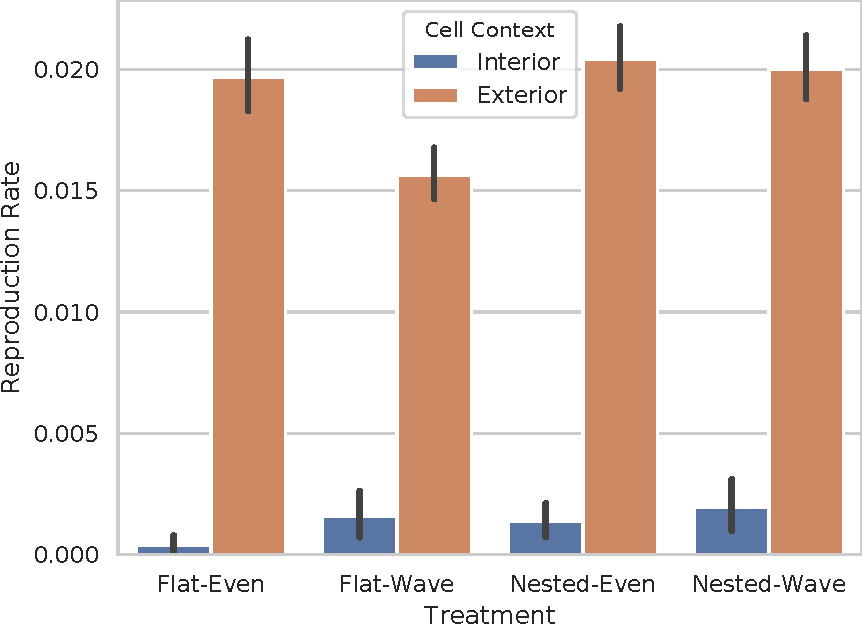
\includegraphics[width=\columnwidth]{img/reproduction/title=reproductive_labor_surrounded+_data_hathash_hash=2400d97af0b49a99+_script_fullcat_hash=d728fc498d889102+_source_hash=53a2252-clean+ext=}

\caption{
Cellular reproduction rates at the interior and exterior of apex-level hereditary groups.
Error bars indicate 95\% confidence.
}
\label{fig:reproduction_surrounded}
\end{center}
\end{figure}


This section contains Figure \ref{fig:reproduction_surrounded}.

\subsection{Resource Sharing} \label{sec:resource-sharing}

\begin{figure*}[!htbp]
\begin{center}

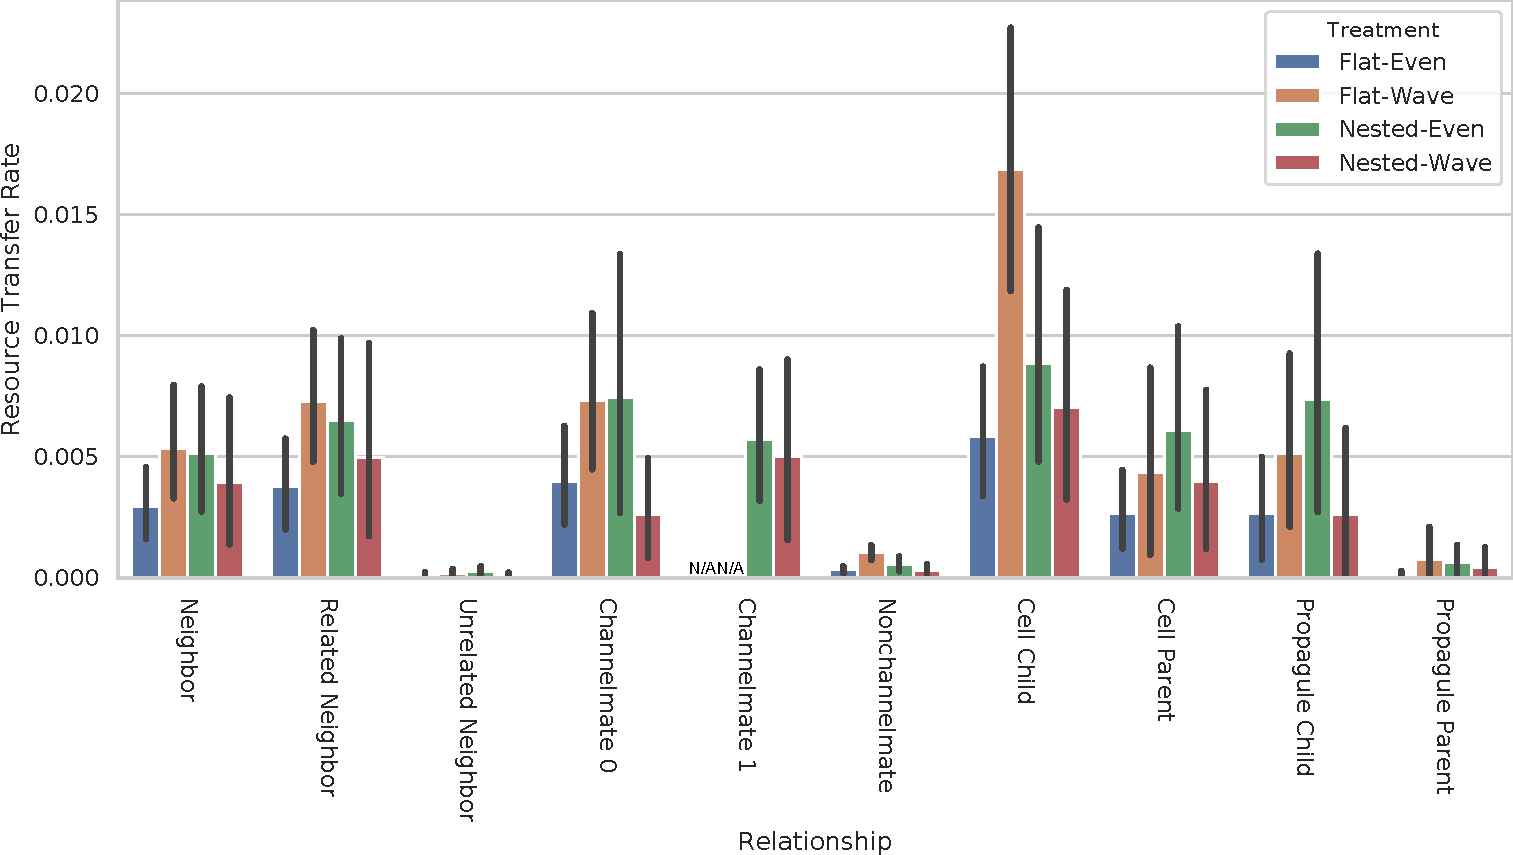
\includegraphics[width=\textwidth]{sharing/title=Resource_Transfer_Rate+_data_hathash_hash=ade957ec08284082+_script_fullcat_hash=e37b8d6f029c9f40+_source_hash=53a2252-clean+ext=}

\caption{
Resource sharing rates across donor-recipient relationships.
Neighbor describes any potential recipient cell.
Related neighbor describes a recipient cell that is a direct cellular progenitor or offspring of the donor, registered to a same hereditary group as the donor, or a member of a hereditary group that is a progenitor or offspring of the donor's.
Unrelated neighbors constitutes all other cells.
Channelmate refers to donor-recipient pairs that are registered to the same hereditary group.
Note that L1 groups are not defined in the flat treatment.
Non-channelmate recipients are not registered to any common hereditary groups with the potential donor.
Cell child and parent describe direct nuclear cell relationships between donor and recipient.
Finally, a propagule child relationship exists when a donor cell is a member of the apex-level hereditary group that directly begat the recipient cell's hereditary group.
A propagule parent relationship describes the reverse, when a recipient cell is a member of the apex-level hereditary group that directly begat the donor cell's hereditary group.
Error bars indicate 95\% confidence.
}
\label{fig:sharing}
\end{center}
\end{figure*}

\begin{figure*}[!htbp]
\begin{center}

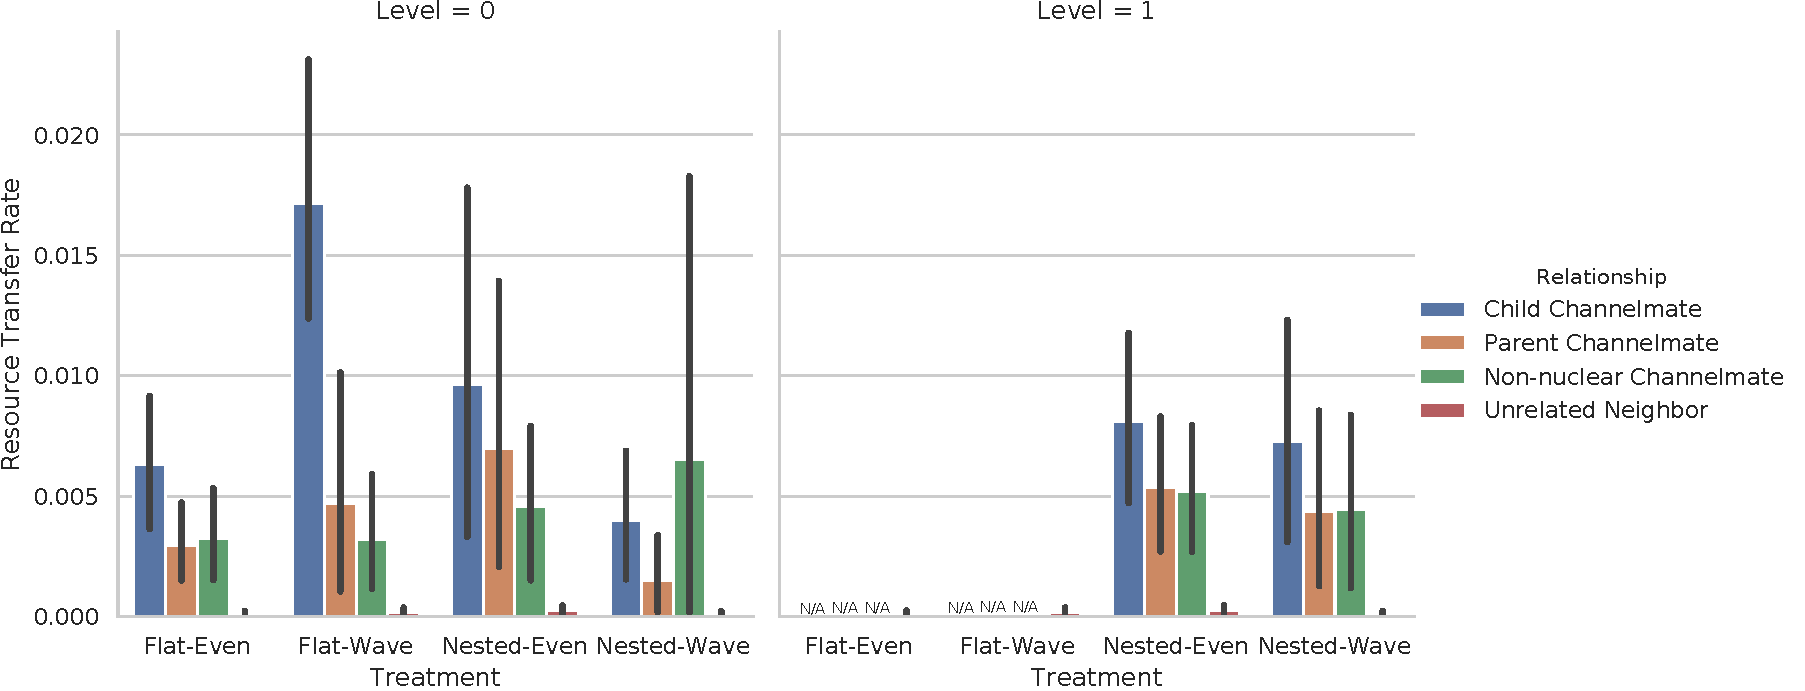
\includegraphics[width=\textwidth]{sharing/title=Resource_Transfer_Rate+_data_hathash_hash=2137e250b9d2b681+_script_fullcat_hash=86edbf4a4e5f34ed+_source_hash=53a2252-clean+ext=}

\caption{
Resource sharing to mutually exclusive sub-categories of hereditary group comrades: cellular child, cellular parent, and neither (``non-nuclear'').
Resource sharing to entirely non-related cells (no cell, hereditary group, or propagule relation) is included for comparison.
Note that L1 hereditary groups are not defined in either of the flat treatments.
Error bars indicate 95\% confidence.
}
\label{fig:sharing_channelmate}
\end{center}
\end{figure*}


Figure \ref{fig:sharing} overviews evolved resource sharing behavior across cellular contexts.

Replicates in the flat-wave treatment exhibit an especially elevated rate of resource sharing to cell children.
This could perhaps be due to an especial selective pressure to convey resource towards the group periphery.

In the Nested-Wave treatment resource was shared at a higher mean rate among L1 hereditary groups than L0 groups.
At face value, this observation appears counterintuitive: why should cells prefer to share with more distant relatives with only one hereditary ID in common as opposed to closer relatives with both hereditary IDs in common?
However, we believe it likely an artifact of replicates where L1 groups were composed of single-cell L0 groups (where no or very few opportunities for L0 resource sharing occurred).

Finally, under all treatments resource was transferred to hereditary group comrades at a significantly higher mean rate than to unrelated neighbors (non-overlapping 95\% CI).
This observation suggests that functional cooperation within hereditary groups might have been a common evolutionary outcome under all four treatments.
However, it could potentially be driven exclusively by resource-sharing between direct cellular kin.

Figure \ref{fig:sharing_channelmate} investigates this possibility by breaking within-group resource sharing apart by cellular kin relation.
In all four treatments, mean sharing to direct-kin hereditary group comrades was indeed greater than to other hereditary group comrades.
This could be due to an evolutionary incentive to favor direct cell kin over other hereditary comrades, group-level selection for asymmetric resource flow achieved by preferential sharing, or some combination of the two.
However, in all four treatments mean sharing to non-direct-kin hereditary group comrades was also significantly greater than resource sharing to unrelated neighbors (non-overlapping 95\% CI).
Thus, all four treatments appear to be sufficient to select for functional cooperation within hereditary groups.

\subsection{Case Study: Cell-Cell Messaging} \label{sec:intergroup}

% \pragmaonce

% adapted from https://www.overleaf.com/learn/latex/Commands
\providecommand{\dissertationelse}[2]{%
% adapted from https://tex.stackexchange.com/a/33577
\ifdefined\DISSERTATION
#1
\else
#2
\fi
}


\begin{figure}[!htbp]
\begin{center}
\begin{minipage}[t]{0.5\linewidth}


% \begin{minipage}[t]{\linewidth}
\centering
\hspace*{\fill}%
\begin{minipage}[t]{0.05\linewidth}
\vspace{0pt} % for alignment
\rotatebox{90}{Messaging}%
\end{minipage}%
\hfill
\begin{minipage}[t]{0.45\linewidth}
\centering
\vspace{0pt} % for alignment
\adjincludegraphics[width=\textwidth, trim={{.66\width} {.66\width} {.0\width} {.0\width}}, clip]{img/knockout/intermessaging-intergroup_border/wildtype/seed=1+title=directional_messaging_viz+treat=resource-wave__channelsense-yes__nlev-two+update=7168+_data_hathash_hash=3895dfa0dd602b4c+_script_fullcat_hash=6b7e0389992dd616+_source_hash=53a2252-clean+ext=}%
\end{minipage}%
\hfill
\begin{minipage}[t]{0.45\linewidth}
\centering
\vspace{0pt} % for alignment
\adjincludegraphics[width=\textwidth, trim={{.66\width} {.66\width} {.0\width} {.0\width}}, clip]{img/knockout/intermessaging-intergroup_border/knockout/seed=1+title=directional_messaging_viz+treat=resource-wave__channelsense-yes__nlev-two+update=7168+_data_hathash_hash=24546cc614406803+_script_fullcat_hash=6b7e0389992dd616+_source_hash=53a2252-clean+ext=}%
\end{minipage}%
\hspace*{\fill}

% \hspace*{\fill}%
% \begin{minipage}[t]{0.05\linewidth}
% \vspace{0pt} % for alignment
% \rotatebox{90}{Parent-Propagule}%
% \end{minipage}%
% \hfill
% \begin{minipage}[t]{0.45\linewidth}
% \centering
% \vspace{0pt} % for alignment
% \adjincludegraphics[width=\textwidth, trim={{.66\width} {.66\width} {.0\width} {.0\width}}, clip]{img/knockout/intermessaging-intergroup_border/wildtype/seed=1+title=directional_propagule_viz+treat=resource-wave__channelsense-yes__nlev-two+update=7168+_data_hathash_hash=3895dfa0dd602b4c+_script_fullcat_hash=8b1f57a580a67198+_source_hash=53a2252-clean+ext=}%
% \end{minipage}%
% \hfill
% \begin{minipage}[t]{0.45\linewidth}
% \centering
% \vspace{0pt} % for alignment
% \adjincludegraphics[width=\textwidth, trim={{.66\width} {.66\width} {.0\width} {.0\width}}, clip]{img/knockout/intermessaging-intergroup_border/knockout/seed=1+title=directional_propagule_viz+treat=resource-wave__channelsense-yes__nlev-two+update=7168+_data_hathash_hash=24546cc614406803+_script_fullcat_hash=8b1f57a580a67198+_source_hash=53a2252-clean+ext=}%
% \end{minipage}%
% \hspace*{\fill}

\hspace*{\fill}%
\begin{minipage}[t]{0.05\linewidth}
\vspace{0pt} % for alignment
\rotatebox{90}{Resource Sharing}%
\end{minipage}%
\hfill
\begin{minipage}[t]{0.45\linewidth}
\centering
\vspace{0pt} % for alignment
\adjincludegraphics[width=\textwidth, trim={{.66\width} {.66\width} {.0\width} {.0\width}}, clip]{img/knockout/intermessaging-intergroup_border/wildtype/seed=1+title=directional_sharing_viz+treat=resource-wave__channelsense-yes__nlev-two+update=7172+_data_hathash_hash=3895dfa0dd602b4c+_script_fullcat_hash=3a1e851383e0ffd4+_source_hash=53a2252-clean+ext=}%
\end{minipage}%
\hfill
\begin{minipage}[t]{0.45\linewidth}
\centering
\vspace{0pt} % for alignment
\adjincludegraphics[width=\textwidth, trim={{.66\width} {.66\width} {.0\width} {.0\width}}, clip]{img/knockout/intermessaging-intergroup_border/knockout/seed=1+title=directional_sharing_viz+treat=resource-wave__channelsense-yes__nlev-two+update=7172+_data_hathash_hash=24546cc614406803+_script_fullcat_hash=3a1e851383e0ffd4+_source_hash=53a2252-clean+ext=}%
\end{minipage}%
\hspace*{\fill}

% \hspace*{\fill}%
% \begin{minipage}[t]{0.05\linewidth}
% \vspace{0pt} % for alignment
% \rotatebox{90}{Resource Stockpile}%
% \end{minipage}%
% \hfill
% \begin{minipage}[t]{0.45\linewidth}
% \centering
% \vspace{0pt} % for alignment
% \adjincludegraphics[width=\textwidth, trim={{.66\width} {.66\width} {.0\width} {.0\width}}, clip]{img/knockout/intermessaging-intergroup_border/wildtype/seed=1+title=stockpile_viz+treat=resource-wave__channelsense-yes__nlev-two+update=7168+_data_hathash_hash=3895dfa0dd602b4c+_script_fullcat_hash=4c8152cbf92e0da6+_source_hash=53a2252-clean+ext=}%
% \end{minipage}%
% \hfill
% \begin{minipage}[t]{0.45\linewidth}
% \centering
% \vspace{0pt} % for alignment
% \adjincludegraphics[width=\textwidth, trim={{.66\width} {.66\width} {.0\width} {.0\width}}, clip]{img/knockout/intermessaging-intergroup_border/knockout/seed=1+title=stockpile_viz+treat=resource-wave__channelsense-yes__nlev-two+update=7168+_data_hathash_hash=24546cc614406803+_script_fullcat_hash=4c8152cbf92e0da6+_source_hash=53a2252-clean+ext=}%
% \end{minipage}%
% \hspace*{\fill}

\vspace{1.0ex}

\hspace*{\fill}%
\begin{minipage}[t]{0.05\linewidth}
\vspace{0pt} % for alignment
\end{minipage}%
\hfill
\begin{minipage}[t]{0.45\linewidth}
\centering
\vspace{0pt} % for alignment
Wild Type
\end{minipage}%
\hfill
\begin{minipage}[t]{0.45\linewidth}
\centering
\vspace{0pt} % for alignment
Messaging Knockout
\end{minipage}%
\hspace*{\fill}

\vspace{1.0ex}

\begin{minipage}{\linewidth}
  \dissertationelse{(a)}{\textbf{(A)}} Phenotype visualizations
  % \label{fig:intermessaging-intergroup_border-phen}
\end{minipage}

% \begin{minipage}[t]{0.8\linewidth}
% \centering
% \vspace{0pt} % for alignment
% \begin{minipage}[b]{\textwidth}
% \includegraphics[width=\textwidth]{img/knockout/intermessaging-intergroup_border/title=sharingfraction+_data_hathash_hash=b0e9f42c3e74cf6a+_script_fullcat_hash=84ce7f4d8802dbab+_source_hash=53a2252-clean+ext=}%
% \caption{Resource sharing}
% \label{fig:intermessaging-intergroup_border-sharing}
% \end{minipage}
% \end{minipage}%
%
% \vspace{1ex}
%
% \hspace*{\fill}%
% \begin{minipage}[t]{0.8\linewidth}
% \centering
% \vspace{0pt} % for alignment
% \begin{minipage}[b]{\textwidth}
% 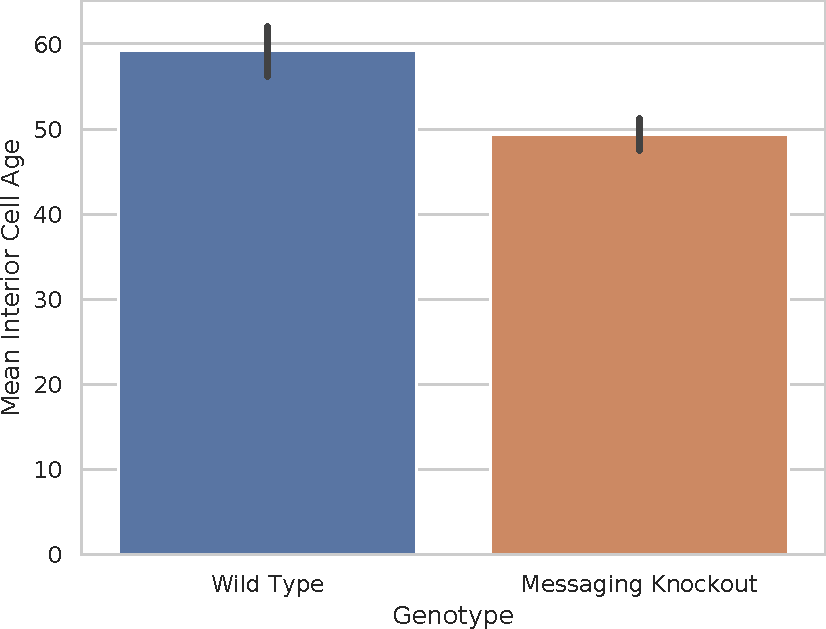
\includegraphics[width=\textwidth]{img/knockout/intermessaging-intergroup_border/title=cellageraw+_data_hathash_hash=ef9f5e984a40fbf6+_script_fullcat_hash=1faec38cdb6bd1de+_source_hash=53a2252-clean+ext=}%
% \caption{Interior cell age}
% \label{fig:intermessaging-intergroup_border-cellage}
% \end{minipage}
% \end{minipage}%
% \hspace*{\fill}

% \end{minipage}%
% \begin{minipage}[t]{\linewidth}
% \centering

% \hspace*{\fill}%
% \begin{minipage}[t]{0.8\linewidth}
% \centering
% \vspace{0pt} % for alignment
% \begin{minipage}[b]{\textwidth}
% \includegraphics[width=\textwidth]{img/knockout/intermessaging-intergroup_border/title=parentage+_data_hathash_hash=974d02d36b7dba1a+_script_fullcat_hash=7ee3d274683ffdb2+_source_hash=53a2252-clean+ext=}%
% \caption{Propagule parent age}
% \label{fig:intermessaging-intergroup_border-pparentage}
% \end{minipage}
% \end{minipage}%
% \hspace*{\fill}

% \vspace{1ex}

\hspace*{\fill}%
\begin{minipage}[t]{0.8\linewidth}
\centering
\vspace{0pt} % for alignment
\begin{minipage}[b]{\textwidth}
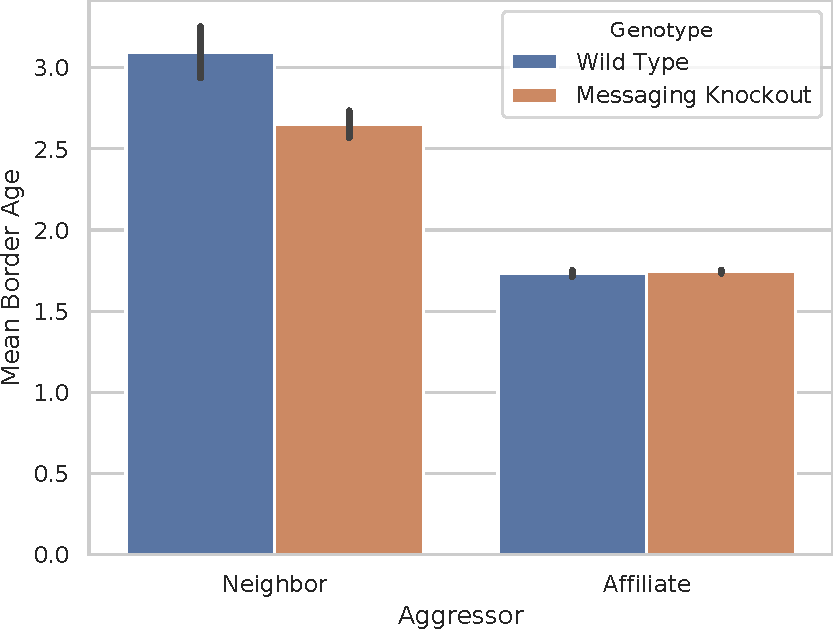
\includegraphics[width=\textwidth]{img/knockout/intermessaging-intergroup_border/title=comboborderage+_data_hathash_hash=8369fa84222d9217+_script_fullcat_hash=c576822d0876c8a8+_source_hash=53a2252-clean+ext=}\\
{\dissertationelse{(b)}{\textbf{(B)}} Border age}
% \label{fig:intermessaging-intergroup_border-borderage}
\end{minipage}
\end{minipage}%
\hspace*{\fill}

\vspace{1ex}

% \hspace*{\fill}%
% \begin{minipage}[t]{0.8\linewidth}
% \centering
% \vspace{0pt} % for alignment
% \begin{minipage}[b]{\textwidth}
% 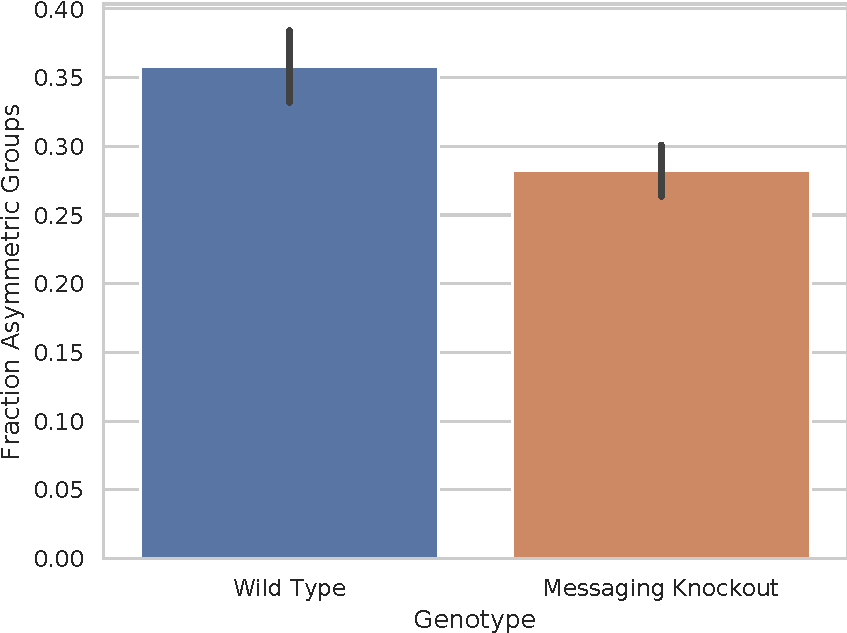
\includegraphics[width=\textwidth]{img/knockout/intermessaging-intergroup_border/title=metabolismasymmetry+_data_hathash_hash=3ce8f7b8474367f3+_script_fullcat_hash=0329612f3b158905+_source_hash=53a2252-clean+ext=}%
% \caption{Asymmetric border metabolism}
% \label{fig:intermessaging-intergroup_border-metabolism}
% \end{minipage}
% \end{minipage}%
% \hspace*{\fill}

\end{minipage}

\caption{
Comparison of wild type strain evolved under the ``Nested-Wave'' treatment and corresponding intercell messaging knockout strain.
Subfigure \dissertationelse{\ref{fig:ko-intermessaging-intergroup_border}a}{\textbf{(A)}} visualizes phenotypic traits in the wild type and knockout strain.
In the messaging visualization, color coding represents the volume of incoming messages.
White represents no incoming messages and the magenta to blue gradient runs from one incoming message to the maximum observed incoming message traffic.
In the resource sharing visualization, this same color coding represents the amount of incoming shared resource.
Solid black borders divide L1 hereditary groups and dotted light gray borders divide L0 hereditary groups.
Subfigure \dissertationelse{\ref{fig:ko-intermessaging-intergroup_border}b}{\textbf{(B)}} quantifies knockout effects on border age.
View an animation of the wild type strain at \url{https://hopth.ru/o}.
View the wild type strain in a live in-browser simulation at \url{https://hopth.ru/d}.
% minipages \ref{fig:intermessaging-intergroup_border-sharing}, \ref{fig:intermessaging-intergroup_border-cellage}, \ref{fig:intermessaging-intergroup_border-pparentage}, \ref{fig:intermessaging-intergroup_border-borderage}, and \ref{fig:intermessaging-intergroup_border-metabolism} quantify knockout effects on various phenotypic traits.
Error bars indicate 95\% confidence.
}
\label{fig:ko-intermessaging-intergroup_border}
% \end{minipage}

\end{center}
\end{figure}


Figure \ref{fig:ko-intermessaging-intergroup_border}\textbf{(A)} compares the cell-cell messaging, resource sharing, and parent-propagule phenotypes between wild type and cell-cell messaging knockout variants of a strain evolved under the Nested-Wave treatment.
Cell-cell messaging volume appears generally uniform in the interiors of hereditary groups, but some group-group borders --- largely, but not entirely parent-propagule interfaces --- manifest somewhat reduced cell-cell messaging overlaid with an alternating motif of elevated cell-cell messaging.
We affirmed the adaptiveness of cell-cell messaging in this strain through competition experiments between wild type and knockout variants ($19/20$; $p < 0.001$; two-tailed Binomial test).
The gene activated by cell-cell messaging in this strain contains a share resource instruction and, indeed, we observed significantly greater net resource sharing in the wild type strain
(%
WT: mean 0.27, S.D. 0.03, $n=20$;
KO: mean 0.23, S.D. 0.02, $n=20$;
$p < 0.001$, bootstrap test
%Figure \ref{fig:intermessaging-intergroup_border-sharing};
non-overlapping 95\% CI%
). %2020-01-06-ll.md
However, that same gene also contains a reproduction-inhibiting instruction, leading us to investigate whether cell-cell messaging could influence a broader set of phenotypic traits.

Cell-cell messaging in the wild type strain appears to be associated with a drawn out hereditary group life history.
The wild-type strain exhibits significantly greater mean cell age
(%
WT: mean 59, S.D. 7, $n=20$;
KO: mean 49, S.D. 4, $n=20$;
$p < 0.001$, bootstrap test%
%Figure \ref{fig:intermessaging-intergroup_border-sharing};
) %2020-01-06-ll.md
and, across propagule-generation events, significantly greater mean parent group age
(%
WT: mean 1055, S.D. 82, $n=20$;
KO: mean 924, S.D. 62, $n=20$;
$p < 0.001$, bootstrap test%
%Figure \ref{fig:intermessaging-intergroup_border-pparentage};
). %2020-01-06-ll.md
This strain exhibits the ``sweep'' life history depicted in Figure \ref{fig:lifecycle}\textbf{(C)}, so propagule generation can be largely or entirely destructive to the parent group.
So, the increase in mean cell age could plausibly be attributable to delayed propagule genesis or, alternatively, delayed propagule genesis could arise from other factors retarding life history.

In this strain, we anecdotally observed that contiguous bands of low cell turnover and anomalous cell-cell messaging volumes frequently arose along parent-propagule borders, but also occasionally between other pairs hereditary groups.
Cell-cell messaging not only enables functional coordination within cellular collectives but could also enable adaptive communication among cellular collectives.
This possibility motivated us to test for non-uniform interactions between hereditary groups that did not share a parent-propagule relationship.

We measured mean border age (equivalent to the youngest age of either flanking cell) along the borders of non-parent-propagule hereditary groups.
Figure \ref{fig:ko-intermessaging-intergroup_border}\textbf{(B)} splits this statistic out between borders that were disrupted either by cells birthed from members of the hereditary groups flanking the border (``affiliate'') or from a member of a third hereditary group (``neighbor'').
In both wild type and knockout strains, there was significantly more recent turnover in the absence of intrusion by a third hereditary group (non-overlapping 95\% CI, bootstrap test).
Restated, borders invaded by a third party were more on average more stable than those perturbed by either of the flanking hereditary groups.

This phenomenon was accentuated in the wild type strain.
Although the wild type strain exhibits slightly higher turnover rates on borders plied by only two groups, borders invaded by a third group are significantly more stale than the knockout strain (non-overlapping 95\% CI, bootstrap test).

Greater age of borders disrupted by a third party would be consistent with a general slowing of turnover as hereditary groups age or reduced resource availability in the presence of a third party.
However, a primitive tit-for-tat policy where a subset of non-parent-propagule hereditary group borders stabilize (until invaded by a third party) could also contribute to such an observation.

So, does the cell reproduction rate fluctuate uniformly across a hereditary group's borders or can reproduction rate differ significantly between a group's borders with different non-parent-propagule neighbor groups at a single time point?
To assess this question, we used Kruskal-Wallis tests (with Bonferroni correction) to screen for hereditary groups with border reproduction rate distributions that differed significantly between neighboring non-propagule-parent hereditary groups.
For each hereditary group, we calculated mean per-border-cell birth rate at the interface of each of its non-propagule-parent neighbor groups.
We collected observations with respect to each neighbor group every eighth update over 256 updates.
Groups with significantly differentiated border reproduction rate distributions occurred in both the wild type and messaging knockout strains.
That is, in both strains, we observed some groups that preferentially expended resource to reproduce at their interfaces with only certain non-parent-propagule hereditary group neighbors.

Again, this phenomenon was accentuated in the wild type strain.
A significantly higher proportion of groups exhibited asymmetric border reproduction rates with non-parent-child groups
(%
WT: mean 0.36, S.D. 0.06, $n=20$;
KO: mean 0.28, S.D. 0.04, $n=20$;
$p < 0.001$, bootstrap test%
). %2020-01-06-ll.md

Messaging between cells registered to different parent-propagule hereditary groups seems unlikely to directly underlie asymmetric border reproduction rates because execution of the gene targeted by messages triggers resource-sharing to the sender, which we seldom observed between non-parent-propagule groups (Figure \ref{fig:ko-intermessaging-intergroup_border}\textbf{(A)}).
So, intercell messaging within hereditary groups most likely underlies this phenomenon.
It seems most plausible that increased incidence of asymmetric border reproduction rates arises as a knock-on effect of the life history retardation effect originally discussed.
Perhaps older, ``full-grown'' hereditary groups arrive at a low-reproduction detente at interfaces with other older, ``full-grown'' hereditary groups while resisting incursion at interfaces with younger, growing hereditary groups.
This would constitute a contextually-expressed tit-for-tat policy, perhaps mediated by cell age or cell generations elapsed from the group's founding propagule cell.

\dissertationonly{\end{levelupfrontiers}}


\end{document}
